In Chapter~\ref{ch:jitter} we saw that there are numerous physical sources of stellar 
jitter. Each contributes to a star's observed radial velocity with a unique structure, 
timescale, and amplitude. Unfortunately, a complete model of 
their cumulative effect is unavailable (we only presented RV jitter 
models from the rotationally modulated magnetic regions). 
The question then becomes \emph{how can we approach the challenge of 
modelling the stellar jitter in RV timeseries with the information that we have on hand?} 
To put it another way, since there is no complete mapping between observable ancillary 
timeseries (see Sect.~\ref{sect:diagnostics}) and RV jitter, what other methods can we 
employ in our modelling. In this chapter we turn our attention to the use of the 
supervised machine learning methods of Gaussian processes to model the RV jitter. \\

\section{An Introduction to Gaussian Processes} \label{sect:gpintro}
Information in the section comes from \cite{rasmussen06} and a great series of 
\href{https://www.youtube.com/playlist?list=PLD0F06AA0D2E8FFBA}{YouTube videos} 
on machine learning and statistics from a user by the name of `mathematicalmonk'. \\

For the problem of detecting planetary signals amid stellar jitter signals whose 
source, and therefore whose manifestation in RV observations is unknown, we require a model 
which is free to conform to the structure of the data residuals after the sought after 
planetary signals have been accounted for. The predictive power of such a model is 
also useful for estimating the jitter signal $y_i$ at unseen values of the independent 
variable time $t_i$. \\

In the frequentist approach, one may assume a particular functional form of the 
model to a particular 
dataset. Once the best-fit parameters of that model have been optimized 
the model can be used to predict the values of $y_i$ at previously unseen epochs $t_i$. 
As an example let's say that we are attempting to model the observed 
photometric variability of a star. If the brightness variations 
appear roughly periodic in time then we might be tempted 
to model the light curve with a purely \emph{sinusoidal function} of the form 

\begin{equation}
\Psi_i = A\sin{(2\pi t_i/P_{\mathrm{rot}}+\phi)},
\end{equation}

\noindent where the model 
has the set of parameters $\mathbf{\Theta}=(A,P_{\mathrm{rot}},\phi)$ representing the 
amplitude, period, and phase of the variability respectively. 
With this model we can estimate the probability of 
obtaining certain values of the star's brightness the next time we go back to the 
telescope to observe its brightness by evaluating the model at those epochs. 
This is great! We have obtained a model that  
can be used for predictive purposes. However, we have assumed a functional form of the 
model which itself can be thought of as a hyperparameter in the modeling process  
and indeed this model may not be completely correct as is often the case for stellar 
photometric variability as the varying lifetimes, contrast, and spatial distribution of 
active regions over consecutive stellar rotation cycles can result in brightness variations 
that are not strictly periodic. In this case a purely sinusoidal function clearly does not 
completely capture the structure present in the star's light curve and we should pursue 
a more complete model. \\

An alternative approach is to assign a prior probability to every possible function 
that could potentially model an input dataset. We'll call this alternative the Bayesian 
approach because it incorporates our prior knowledge of what can reasonably model our 
training dataset and potentially any unseen data. But computational 
restrictions and \emph{my} finite lifetime dictates that I cannot possibly evaluate 
\emph{every possible function}. Instead we shall use a non-parametric Gaussian 
process (GP) regression model to provide a probabalistic estimate of the `best-fit'
function to our data. GP regression modeling is a method of supervised learning 
wherein a training dataset is used to train the hyperparameters of the model. The 
GP with its unique set of hyperparameters forms a predictive distribution from which we 
can sample in order to make predictions at new epochs. 
A GP can also be thought of as a Bayesian approach to fitting a dataset in a 
non-parametric way. This implies that we do not consider a specific functional 
form of the model to the data as we did when modelling a star's brightness variations 
with a sinusoidal function. Instead the only model prior that we implement is with 
regards to \emph{how the data are correlated with each other}. In this way, 
\emph{the data itself 
will determine the shape of the model allowing us to make fewer prior assumptions 
regarding its functional form  
thus giving more freedom to the model compared to when its functional form was 
fixed.} This makes Gaussian progress regression categorically a machine learning 
technique and one that is well suited to modelling the complex stocastic processes giving
rise to RV jitter. \\

\subsection{Mathematical Representation}
GPs are commonly used in many scientific fields 
outside of astronomy and have a robust mathematical foundation. 
We begin with the formal definition of a GP: \\

\textbf{Definition}: For any set $\mathbf{S}$, a Gaussian process on $\mathbf{S}$ is a set 
of random variables $\{\mathbf{Z}_t: t \in \mathbf{S}\}$ such that $\forall \hspace{4pt} n \in \mathbb{N}$ 
and $\forall \hspace{4pt} t_1,\dots,t_n \in \mathbf{S}$, the vector $\mathbf{Z}=(Z_1,\dots,Z_n)$ is a 
multivariate Gaussian. \\

%https://www.youtube.com/playlist?list=PLD0F06AA0D2E8FFBA mathematicalmonk
\noindent In essence, \emph{a GP is any set of random variables for which any finite subset follow 
a Gaussian distribution}. \\

The one dimensional Gaussian (or normal) distribution is 

\begin{equation}
\mathcal{N}(x;\mu \sigma) = \frac{1}{\sqrt{2\sigma^2\pi}}\exp{\left( -\frac{(x-\mu)^2}{2\sigma^2} \right)}.
\label{eq:1dgaussian}
\end{equation}

\noindent This is the Gaussian probability density function in one dimension 
of the random variable $x$ parameterized 
by its scalar mean $\mu$ and scalar variance $\sigma^2$. Examples of Gaussian PDFs with 
various $(\mu,\sigma)$ are shown in Fig.~\ref{fig:gaussians}. \\

\begin{figure}
\centering
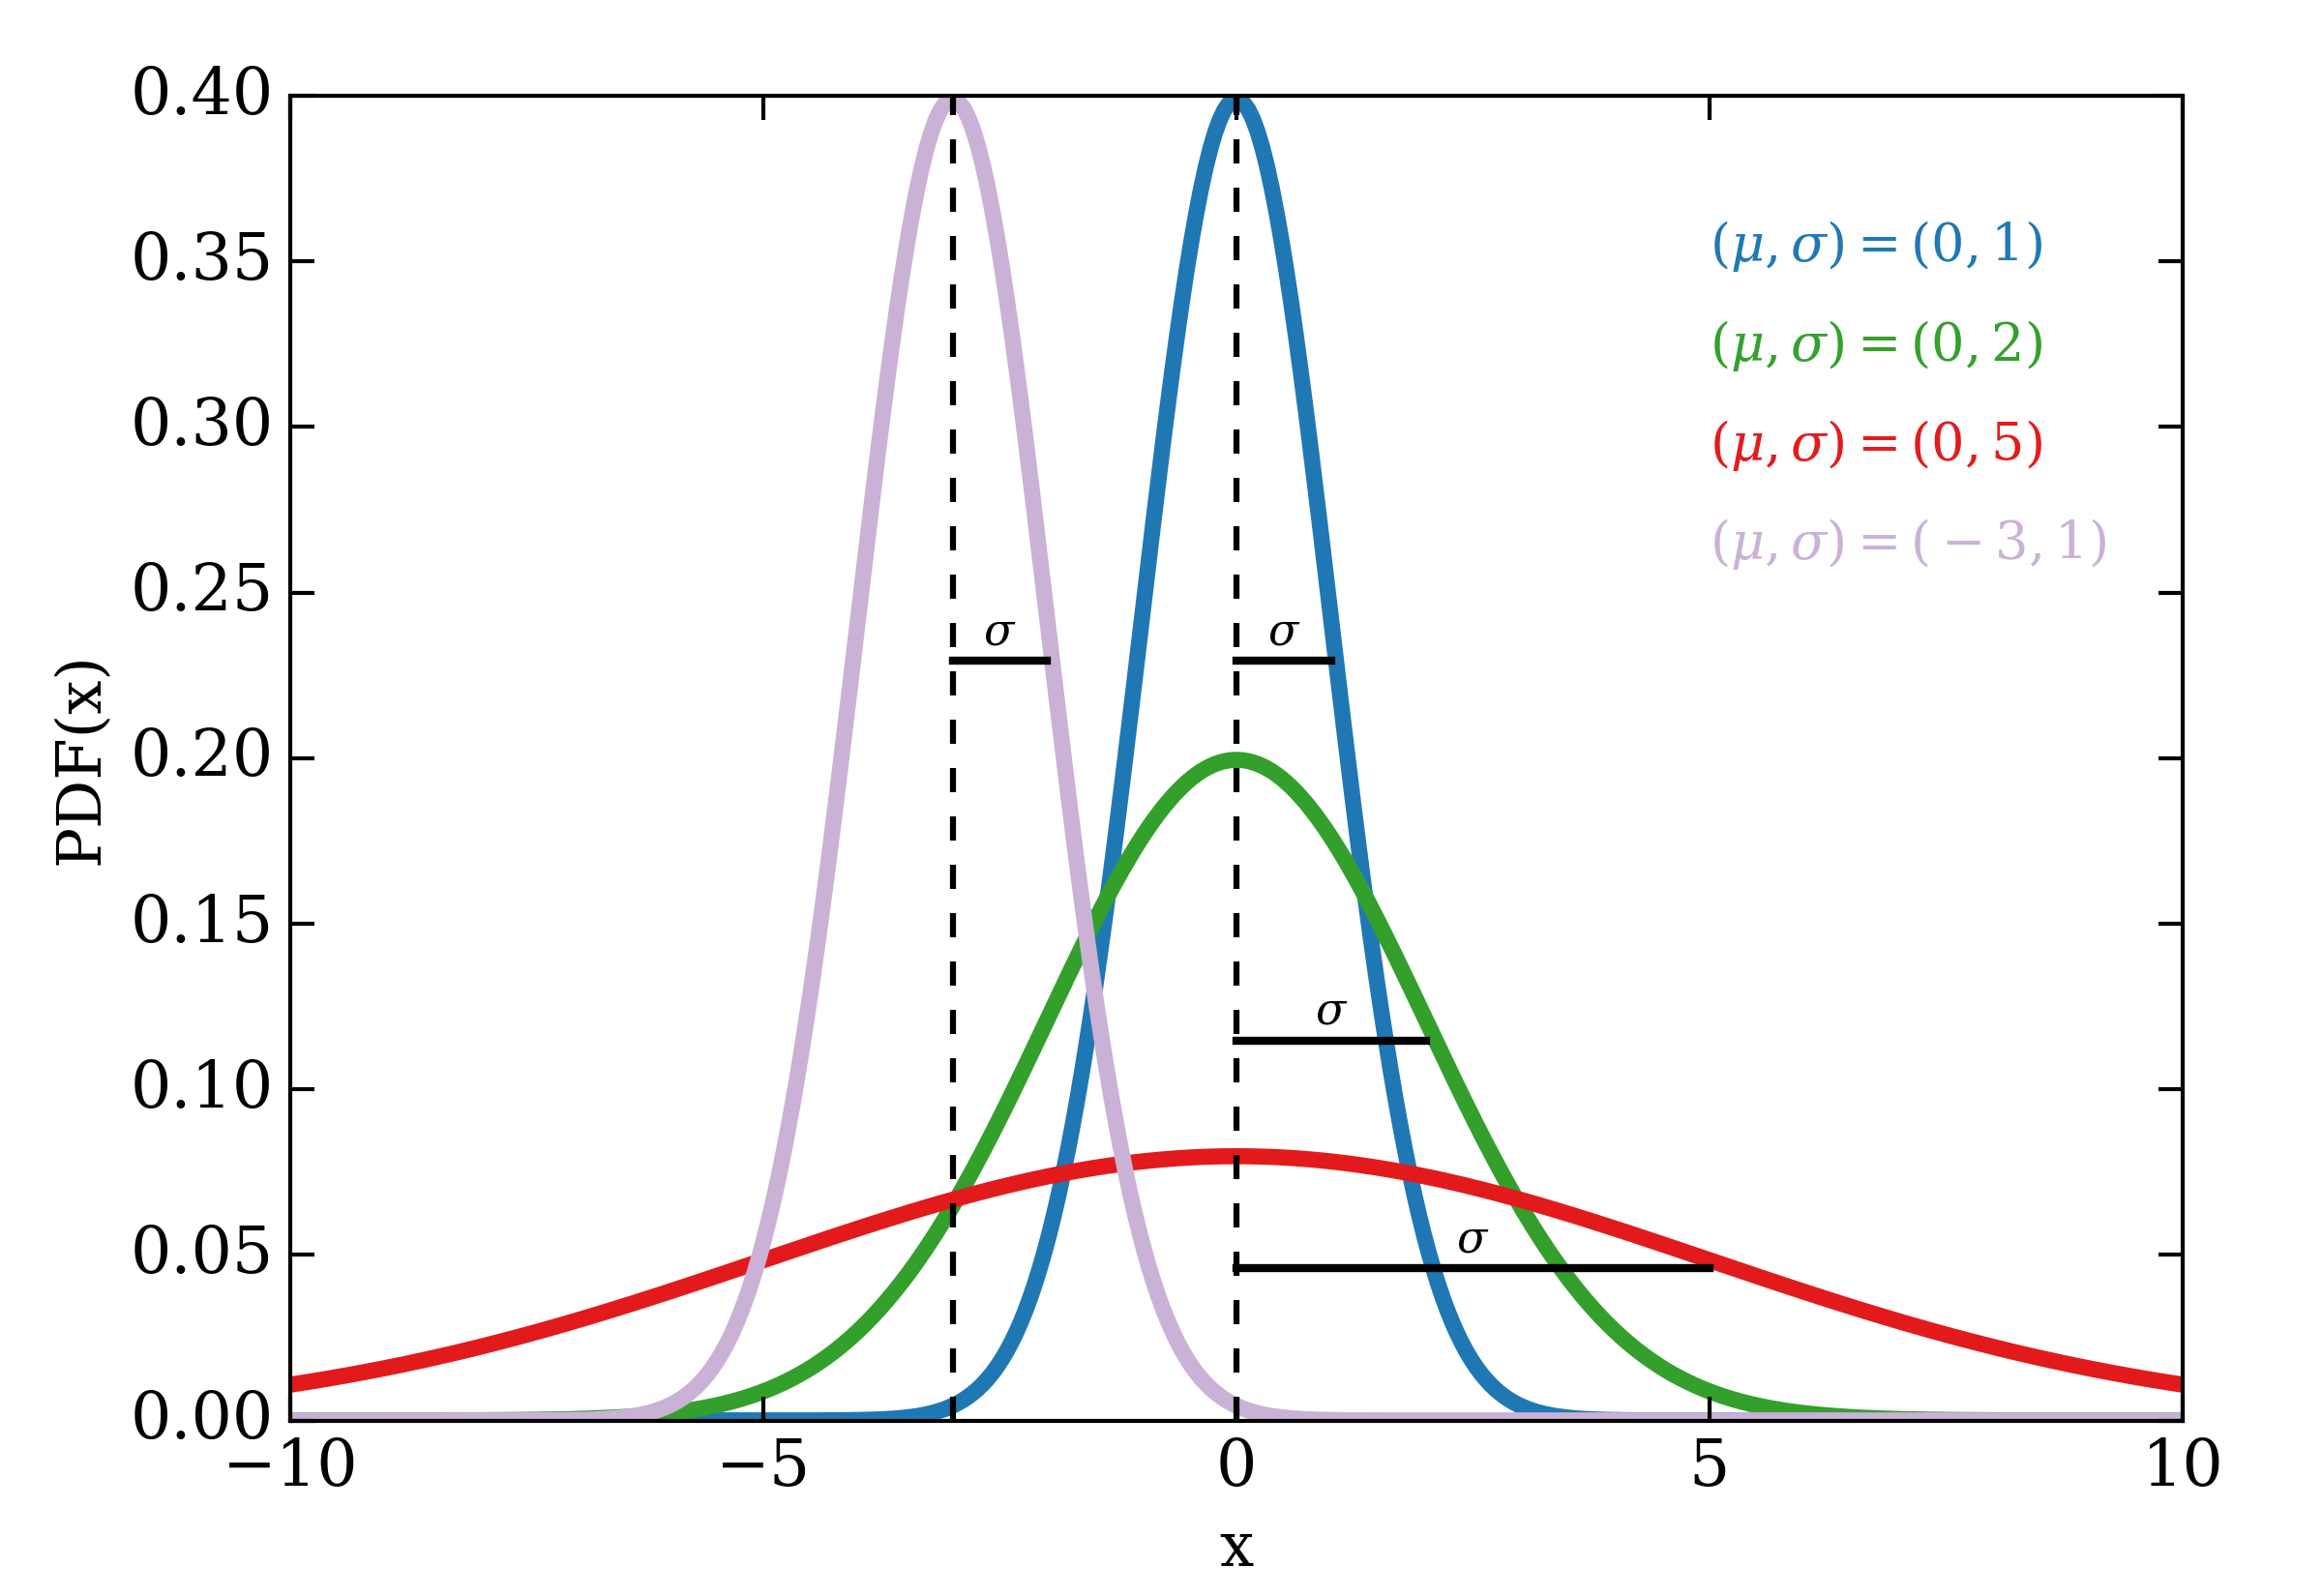
\includegraphics[scale=.45]{figures/gaussians.png}
\caption{A suite of Gaussian probability density functions for various mean and 
standard deviations ($\mu,\sigma$). 
\label{fig:gaussians}}
\end{figure}

The one dimensional (univariate) Gaussian distribution can be generalized to a higher 
dimension $k > 1$ with a mean $k$-vector $\boldsymbol{\mu}$ and a $k \times k$ 
symmetric, positive semidefinite\footnote{A $k \times k$ matrix $\mathbf{M}$ of real numbers 
is positive semidefinite if the scalar value $\mathbf{x}^{\mathrm{T}}\mathbf{M} \mathbf{x} \geq 0$, $\forall$ 
non-zero vector $\mathbf{x}$. 
$\mathbf{M}$ is positive definite if $\mathbf{x}^{\mathrm{T}}\mathbf{M} \mathbf{x} > 0$.} 
covariance matrix $\mathbf{K}$. 
A multivariate normal distribution is said to be non-degenerate when the covariance 
matrix $\mathbf{K}$ is positive definite. In this case we can write 
the multivariate normal probability density function as 

\begin{equation}
\mathcal{N}(\mathbf{x}; \boldsymbol{\mu}, \mathbf{K}) = \frac{1}{\sqrt{(2 \pi)^{k} \mathrm{det} \mathbf{K}}}
\exp{\left( -\frac{1}{2} (\mathbf{x} - \boldsymbol{\mu})^{\mathrm{T}} \mathbf{K}^{-1} (\mathbf{x} - 
\boldsymbol{\mu}) \right)}
\label{eq:kdgaussian}
\end{equation}

\noindent where $\mathbf{x}$ is the $k$-dimensional vector of independent variables, 
and the linear algebra operations `det', `T', and `-1' refer to the determinant, transpose, and
inverse respectively. Note that when $k=1$, $\boldsymbol{\mu} \to \mu$ and the $1\times 1$ matrix 
$\mathbf{K} \to \sigma^2$ such that Eq.~\ref{eq:kdgaussian} simply 
reduces to the univariate Gaussian in Eq.~\ref{eq:1dgaussian}. \\

By its definition a GP prior can be represented as a $k$-dimensional multivariate Gaussian
distribution over functions:

\begin{equation}
\text{P} = \mathcal{N}(\mathbf{x}; \boldsymbol{\mu}, \mathbf{K}).
\label{eq:multvar}
\end{equation}

\noindent By exploiting the properties of Gaussian distributions this GP prior has a
well-defined maximum (i.e. its mean function) and confidence intervals often expressed as
the $1\sigma$ dispersion about the mean function. 

From the GP prior one wishes to arrive at a predictive GP posterior distribution conditioned on some
data. Given a training dataset $\mathbf{y}$ evaulated at $\mathbf{x}$, and a set of hyperparameters
which describe the data's covariance structure (see Sect~.\ref{sect:covariance} for more details on
the covariance), the predictive mean of the GP at $N'$ previously unseen values of the independent variable
$\mathbf{x'}$ can be calculated via

\begin{equation}
\mathbf{M} = \mathbf{K}(\mathbf{x'}, \mathbf{x}) \mathbf{K}(\mathbf{x},\mathbf{x})^{-1} \mathbf{y}.
\label{eq:predmean}
\end{equation}

\noindent Similarly the $N' \times N'$ covariance matrix of the predictive GP can be calculated via

\begin{equation}
\mathbf{C} = \mathbf{K}(\mathbf{x'}, \mathbf{x'}) - \mathbf{K}(\mathbf{x'}, \mathbf{x})
\mathbf{K}(\mathbf{x}, \mathbf{x})^{-1} \mathbf{K}(\mathbf{x'}, \mathbf{x})^T
\label{eq:predsig}
\end{equation}


\subsubsection{Quick example}
The simplest non-trivial example of a GP is known as `random lines' or `random 
planes' in one dimension. For the set of real numbers $\mathbf{S}=\mathbb{R}$, 
we define the set 
$Z_t =tW$ where $W \sim \mathrm{N}(0,1) \in \mathbb{R}$ is a standard normal 
random variable; $W$ is drawn from the univariate Gaussian with zero mean and unit variance. 
In this way, for each random draw of $W$, $Z_t$ is a `random line' with slope $W$ and 
is a set of random variables on the set $\mathbf{S}$ containing all real values of $t$. 
Because $Z_t=tW$ and $W$ is Gaussian distributed, 
by the affine invariant property of a multivariate Gaussian (here we're just considering 
$k=1$), $Z_t$ is also multivariate Gaussian and therefore satisfies the above definition 
of a GP on $\mathbf{S}$. \\

To illustrate this, 
for the subset of $\mathbf{S}$ containing $t \in [0,1]$, we sample $W$ and plot 
$Z_t$ in Fig.~\ref{fig:randomlines}. Each draw represents a GP process on the 
subset $[0,\dots,1]$ which we can see, after a significant (but still finite) number of 
draws, form random lines which are \emph{approximately} 
Gaussian distributed. In the limit of 
an infinite number of draws, the set of random lines would be \emph{absolutely} Gaussian 
distributed. \\

\begin{figure*}
\centering
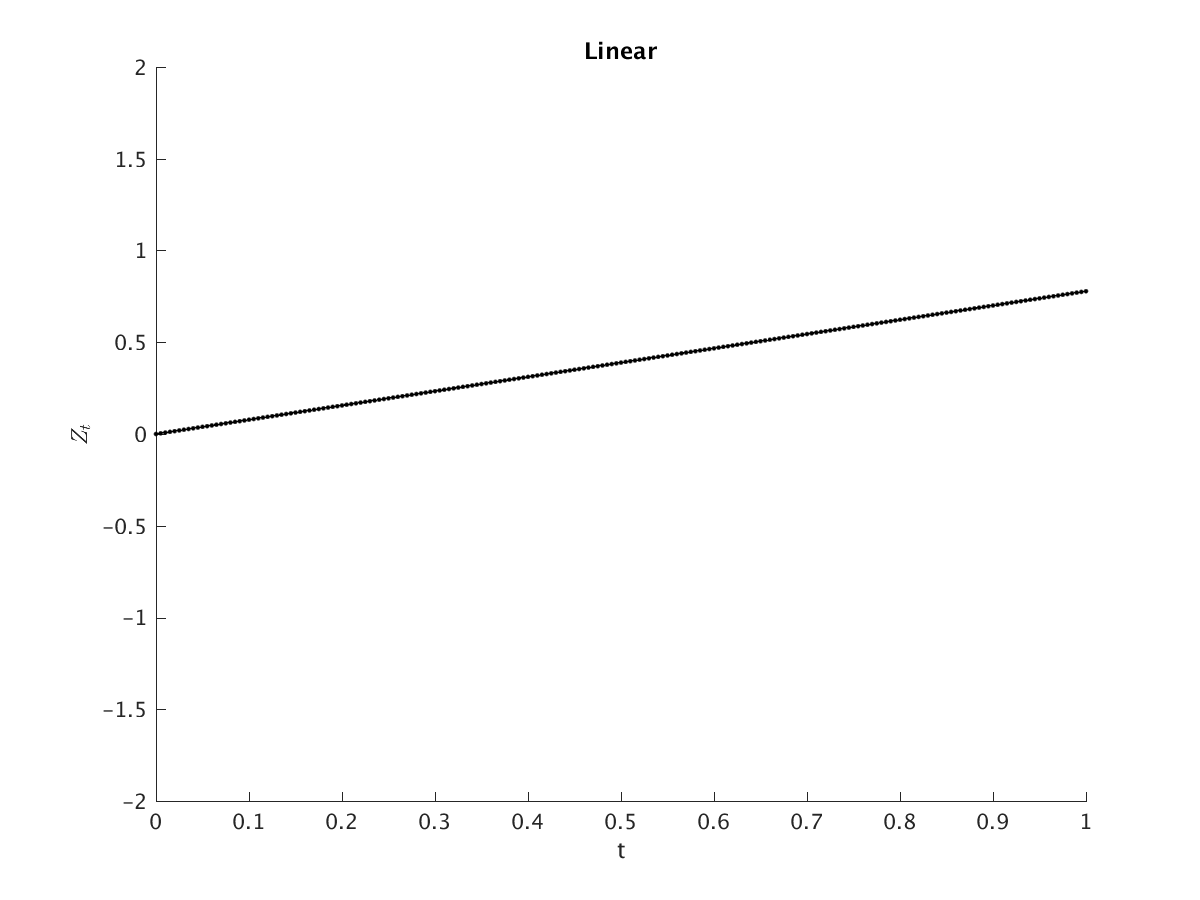
\includegraphics[scale=.45]{figures/linear1.png}
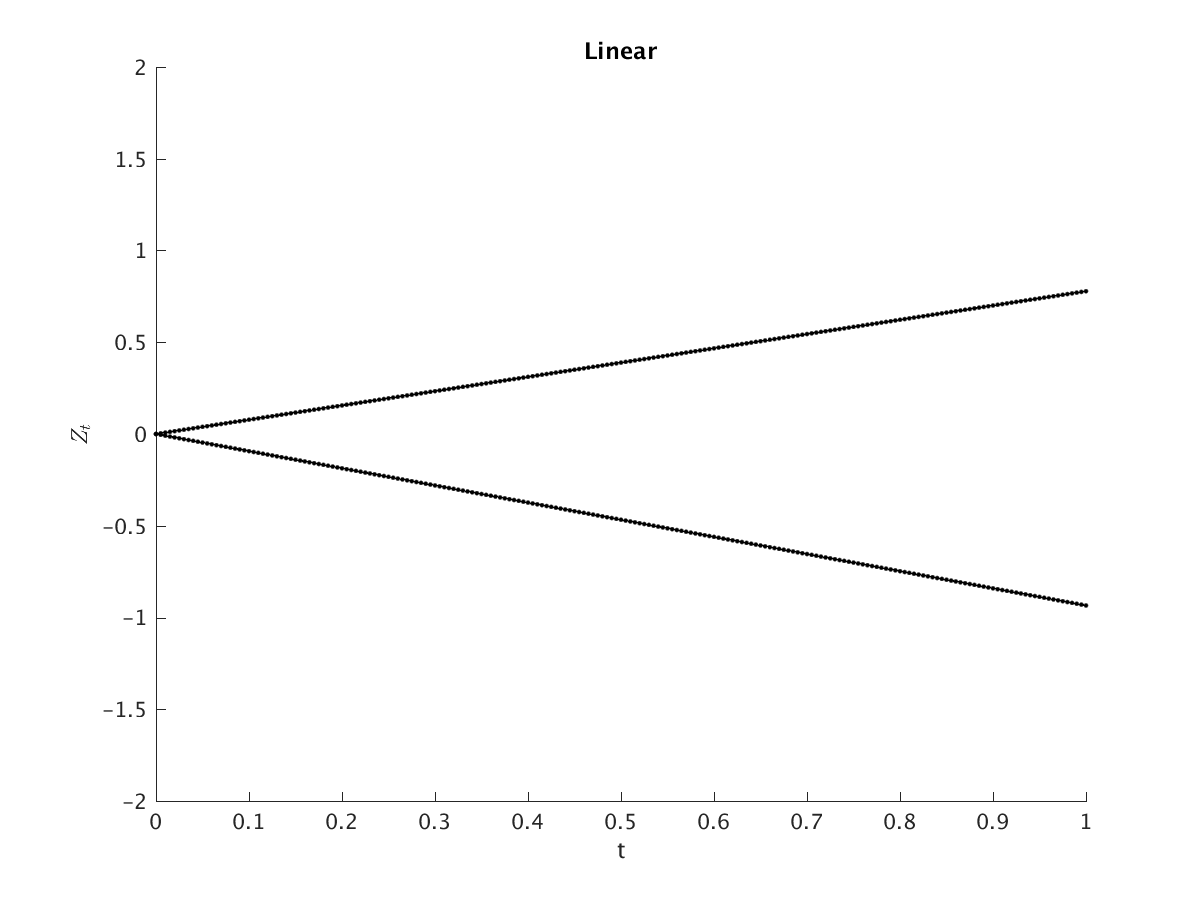
\includegraphics[scale=.45]{figures/linear2.png}
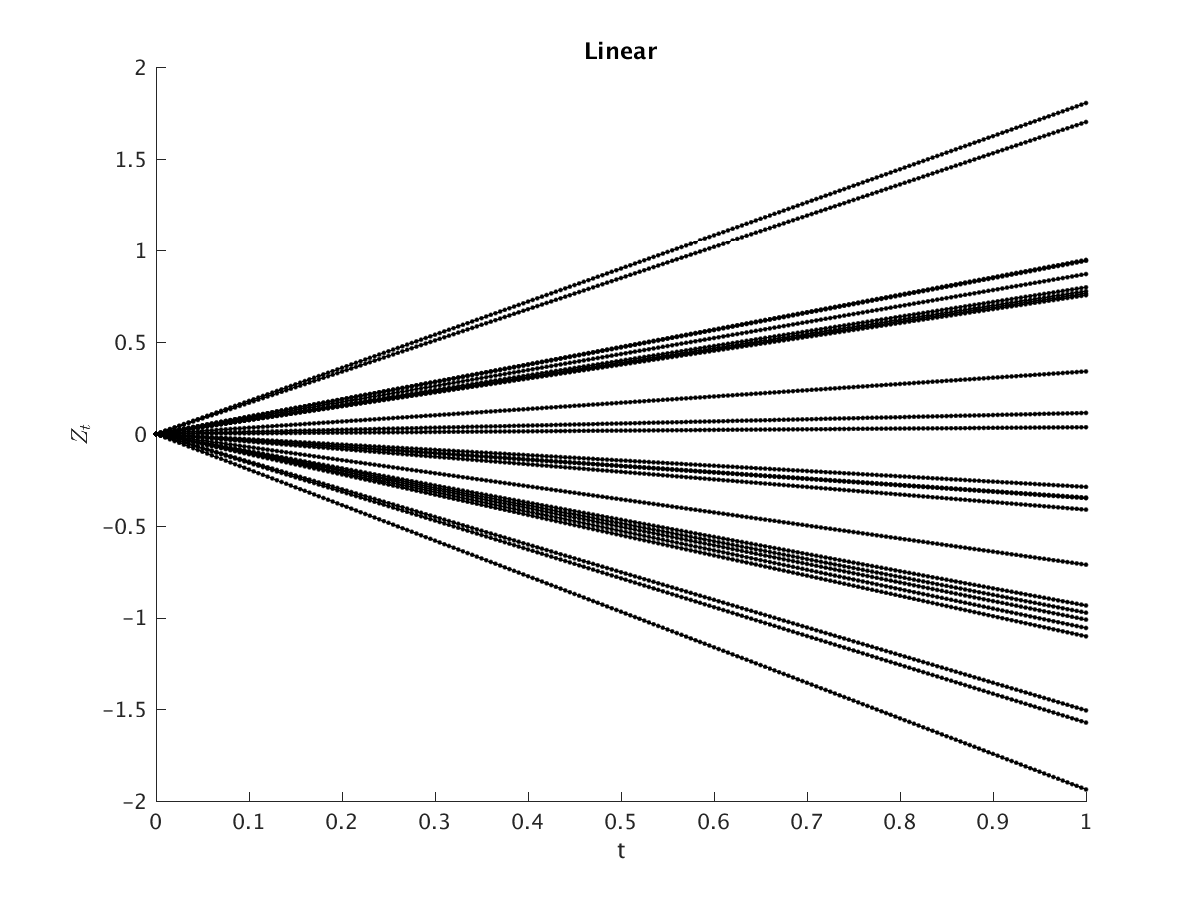
\includegraphics[scale=.45]{figures/linear25.png}
\caption{Successive draws from the Gaussian process $Z_t=tW$ on $t \in [0,1]$ 
where $W$ is a normally distributed random variable with zero mean and unit variance. 
\label{fig:randomlines}}
\end{figure*}


\subsubsection{GP Existence}
When defining a GP on the points $t \in \mathbf{S}$, the process must be 
specified by a mean function $\mu(t)$ 
and covariance function $k(t,t')$. We state the following 
important theorem regarding the existence of GPs without proof: \\

\textbf{Theorem}: 
For any set $\mathbf{S}$, any mean function $\mu(t): \mathbf{S} \to \mathbb{R}$ and 
any covariance function $k(t,t'): \mathbf{S} \times \mathbf{S} \to \mathbb{R}$, 
$\exists$ a Gaussian 
process $\mathbf{Z}_t$ on $\mathbf{S}$ such that the expected value of $Z_t$ is 
equal to $\mu(t)$ with 
cov$(Z_s,Z_t) = k(s,t)$, $\forall \hspace{4pt} s,t \in \mathbf{S}$. \\

This implies that for any appropriate choice of $\mu(t)$ and $k(t,t')$, we can construct 
a valid GP. 
In the case of radial velocities, this is beneficial as we can prescribe a non-zero 
mean function 

\begin{equation}
\mu(t) = \sum_{i=1}^{N} \mathrm{K}_i(t) 
\label{eq:keps}
\end{equation}

\noindent for any number of keplarians $N \ge 0$ (K$_i=v(t)$; see Eq.~\ref{eq:rv}), adopt a 
valid covariance 
function to describe the additive stellar jitter, and we are guaranteed that 
there exists a GP which describes the dataset in this way.

\section{GP Formalism} \label{sect:gpformalism} 
As we have seen, a GP is specified by a mean function $\mu(t)$ and 
covariance function $k(t,t')$. The independent variable time 
is typically written as the 1d vector $\mathbf{t}=(t_1,\dots,t_N)$ where $N$ is the 
number of measurements. Hence the mean function should also be written in vector 
notation: $\mu(t) \to \boldsymbol{\mu}(\mathbf{t})$. 
The vector of measurements is $\mathbf{y}=(y_1,\dots,y_N)$ with 
uncertainties $\boldsymbol{\sigma}=(\sigma_1,\dots,\sigma_N)$. The 
covariance for the \emph{residual} measurements $\mathbf{r}(\mathbf{t})$ is then 
specified after the removal of the GP mean function; 
$\mathbf{r}(\mathbf{t}) = \mathbf{y}(\mathbf{t}) - \boldsymbol{\mu}(\mathbf{t})$. 
The first step in constructing a GP jitter model is to prescribe the way in 
which the data are correlated in time via the covariance function.

\subsection{Covariance Functions} \label{sect:covariance}
The covariance function describes how each measurement in the residual 
timeseries is correlated with every other measurement. Specifically, 
the amplitude of the correlation between two observations taken at different 
epochs $t_i$ and $t_j$ only depends on the absolute time difference between 
them $|t_i-t_j|$, with the maximum correlation occurring when $i=j$. 
The correlation properties of a dataset are contained within the $N \times N$ 
covariance matrix 

\begin{equation}
\mathbf{K}_{i,j} = \sigma_i^2 \delta_{i,j} + k(t_i, t_j), \label{eq:Kmatrix}
\end{equation}

\noindent where $\sigma_i$ is the uncertainty on the $i^{\mathrm{th}}$ measurement 
$y_i$, $\delta_{i,j}$ is the Kronecker delta function, and $k$ is the prescribed 
covariance function. The covariance function is chosen by the supervisor and each 
functional form of $k(t_i,t_j)$ has a unique set of model hyperparameters. \\

There are a number of covariance functions (alternatively referred to as kernel 
functions) commonly used to describe how a timeseries is correlated. Some of the 
most commonly used kernel functions are described below.

\begin{enumerate}
\item \textbf{White Kernel}: is the simplest possible kernel function as all 
off-diagonal elements of the covariance matrix $\mathbf{K}$ are set to zero; 
$k(t_i, t_j) = 0$, $\forall i,j \in [1,N]$. 
Data described by this covariance function are in fact uncorrelated; 
so-called \emph{white noise}. The corresponding covariance matrix 
is therefore diagonal with diagonal elements $K_{i,i} = \sigma_i^2$. 
%Fig.~\ref{fig:linear} shows random samples of this white GP with constant variance 
%$\sigma^2$. \\

\item \textbf{Squared Exponential}: is perhaps the most widely used covariance 
function. This kernel specifies that measurements made closely in time are more 
strongly correlated 
than measurements which are distant in time. The correlation timescale $\lambda$ is a 
hyperparameter of the kernel 

\begin{equation}
k(t_i, t_j) = a^2 \exp{\left(-\frac{|t_i-t_j|^2}{2\lambda^2} \right)}.
\end{equation}

\noindent The squared exponential kernel clearly has two hyperparameters 
$\mathbf{\Theta} = \{a, \lambda \}$ where $a$ is the amplitude of the 
correlations. Three samples from a GP with a squared exponential covariance function 
are shown in Fig.~\ref{fig:sqexp} along with the corresponding covariance matrix 
and the 1d covariance function as a function of the absolute time difference.

\begin{figure}
\centering
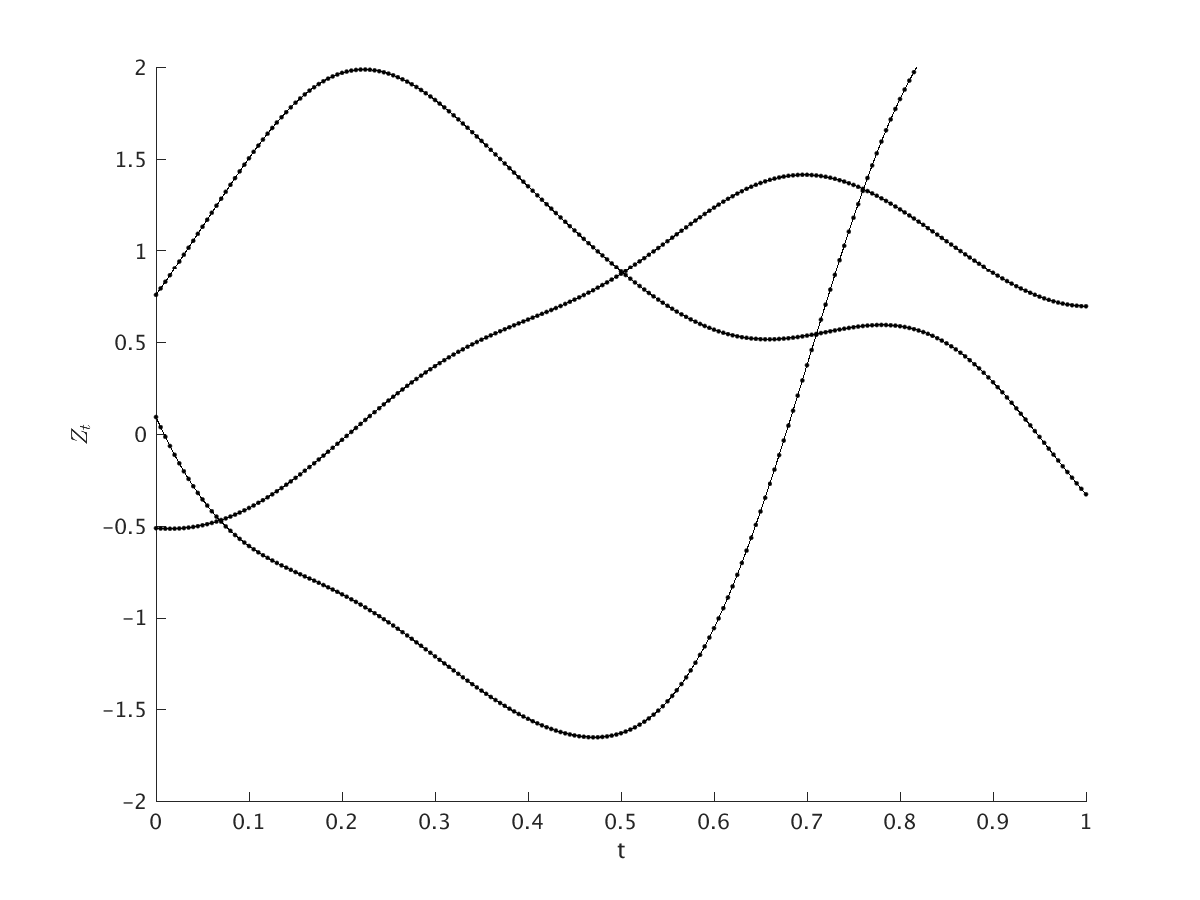
\includegraphics[scale=.5]{figures/sqexp3.png}
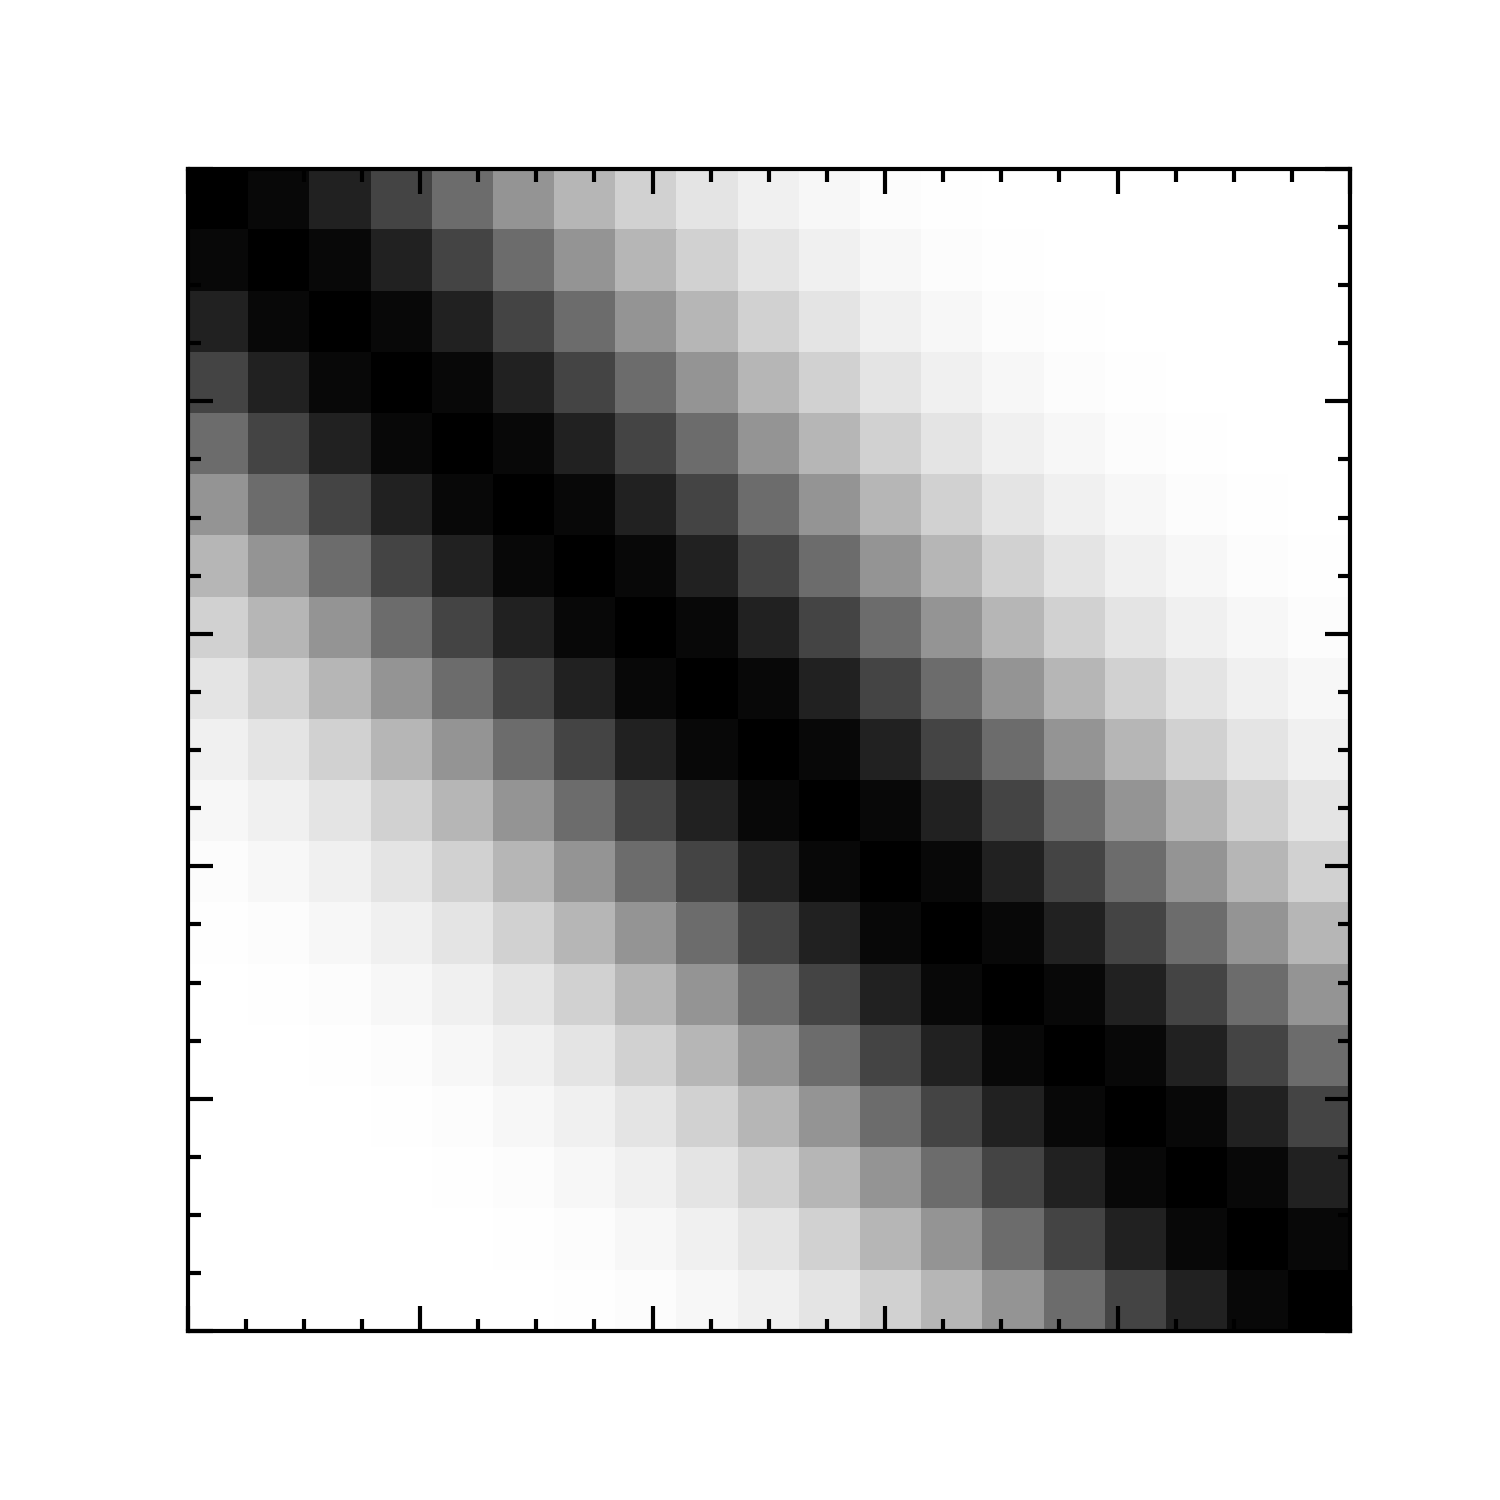
\includegraphics[scale=.4]{figures/covariancematrix_sqexp.png}
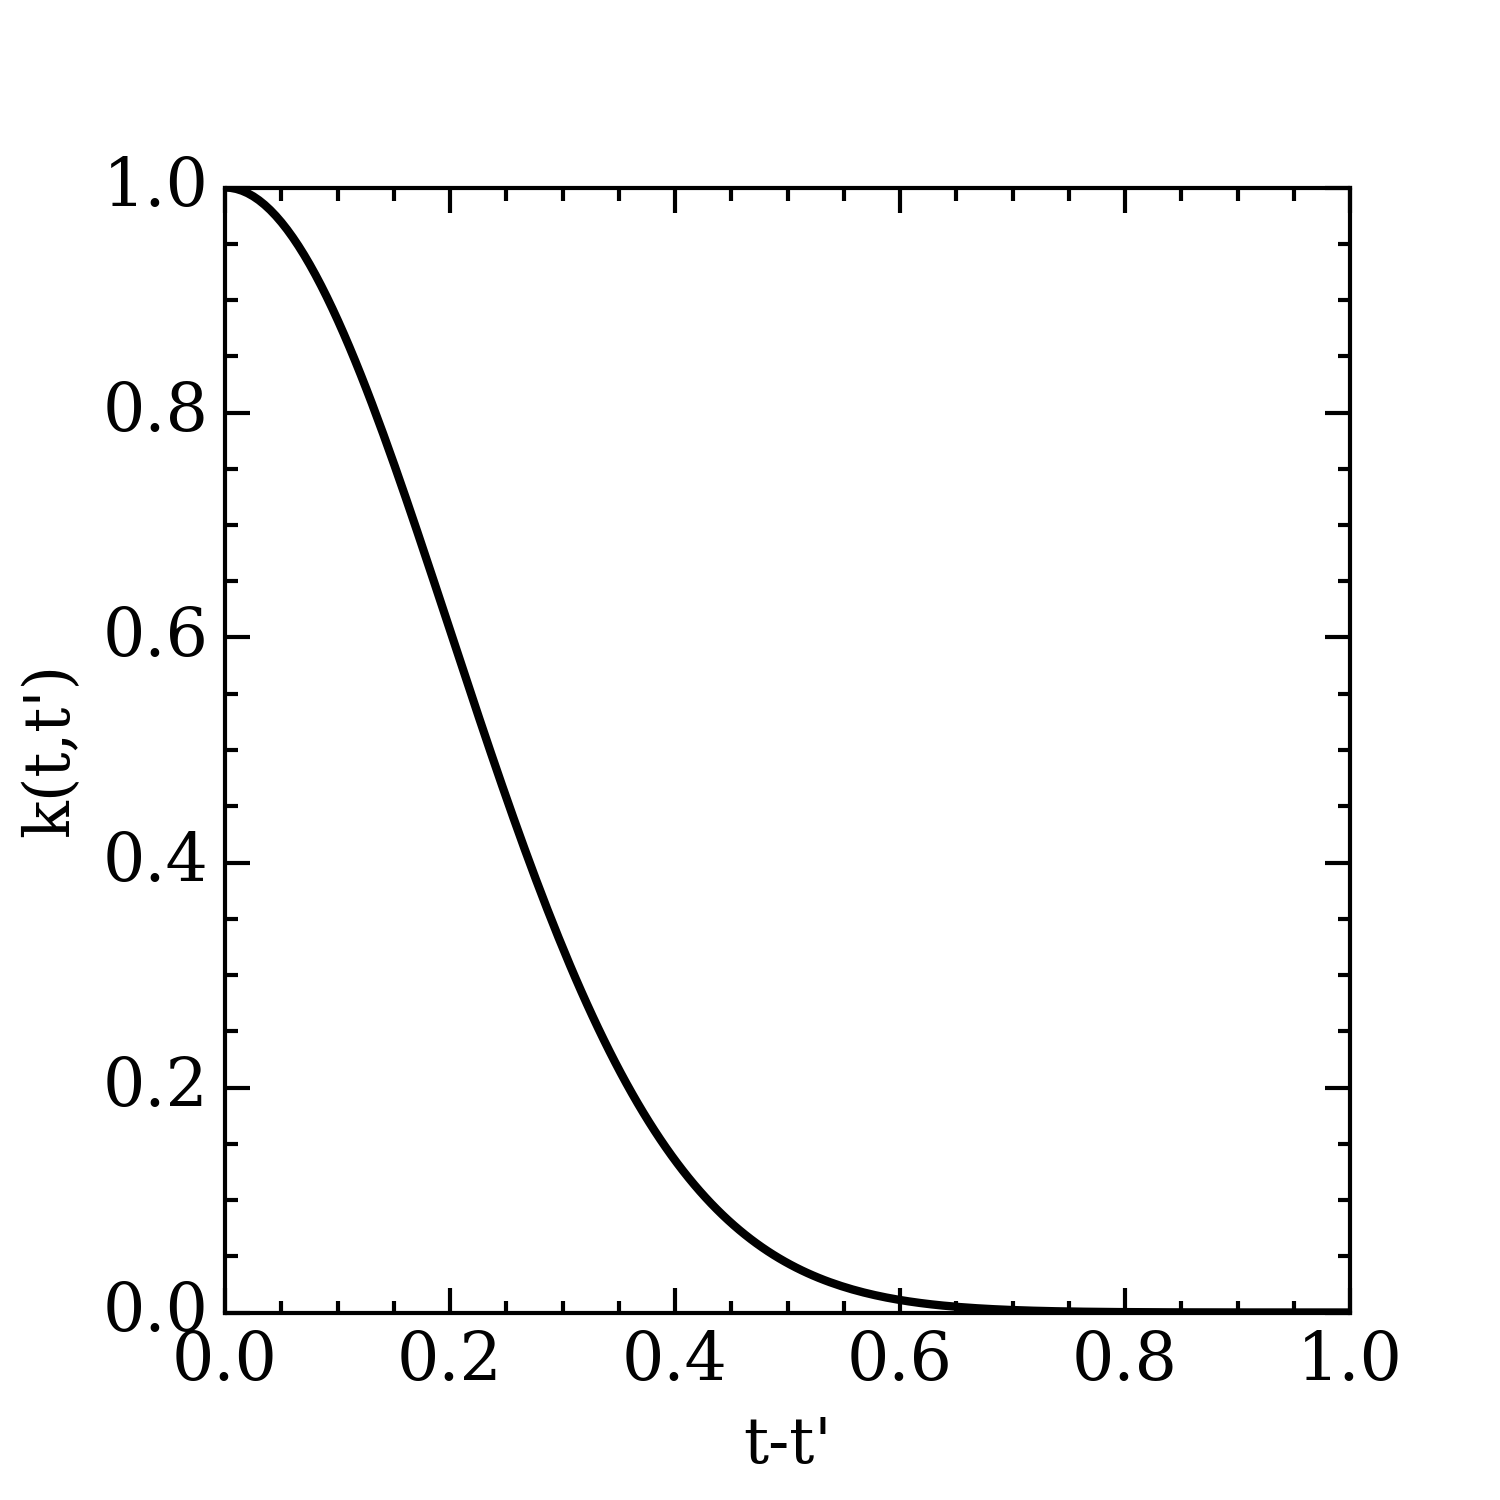
\includegraphics[scale=.4]{figures/kernel_sqexp.png}
\caption{\emph{Top panel}: three samples from a GP with zero mean and a 
squared exponential covariance function. \emph{Lower left panel}: the 
covariance matrix $\mathbf{K}$ for the same squared exponential kernel where 
dark bins denote stronger correlations. 
\emph{Lower right panel}: the same squared exponential covariance function 
as a function of the absolute time difference. 
In all panels $\mathbf{\Theta} = \{a, \lambda \}= \{1, 0.2\}$.
\label{fig:sqexp}}
\end{figure}

\item \textbf{Periodic}: is strictly periodic in time. The correlation is strongest for 
measurements whose absolute time difference is $nP$ where $P$ is the timescale of the 
correlations and $n \in \mathbb{Z}$.\footnote{If you're like me and can never remember, 
$\mathbb{Z}$ is the set of integers.} The covariance function is 

\begin{equation}
k(t_i,t_j) = a^2 \exp{\left( -\Gamma \sin^2{\left[ \frac{\pi |t_i-t_j|}{P} \right]} \right)}
\end{equation}

\noindent where again $a$ is the amplitude of the correlations, $\Gamma$ is a coherence 
parameter or simply the amplitude of the periodicity, and $P$ is the aforementioned 
period of the 
correlations; $\mathbf{\Theta}=\{a,\Gamma,P \}$. Three samples from a GP with a periodic 
covariance function are shown in Fig.~\ref{fig:periodic} along with the corresponding 
covariance matrix and kernel function.

\begin{figure}
\centering
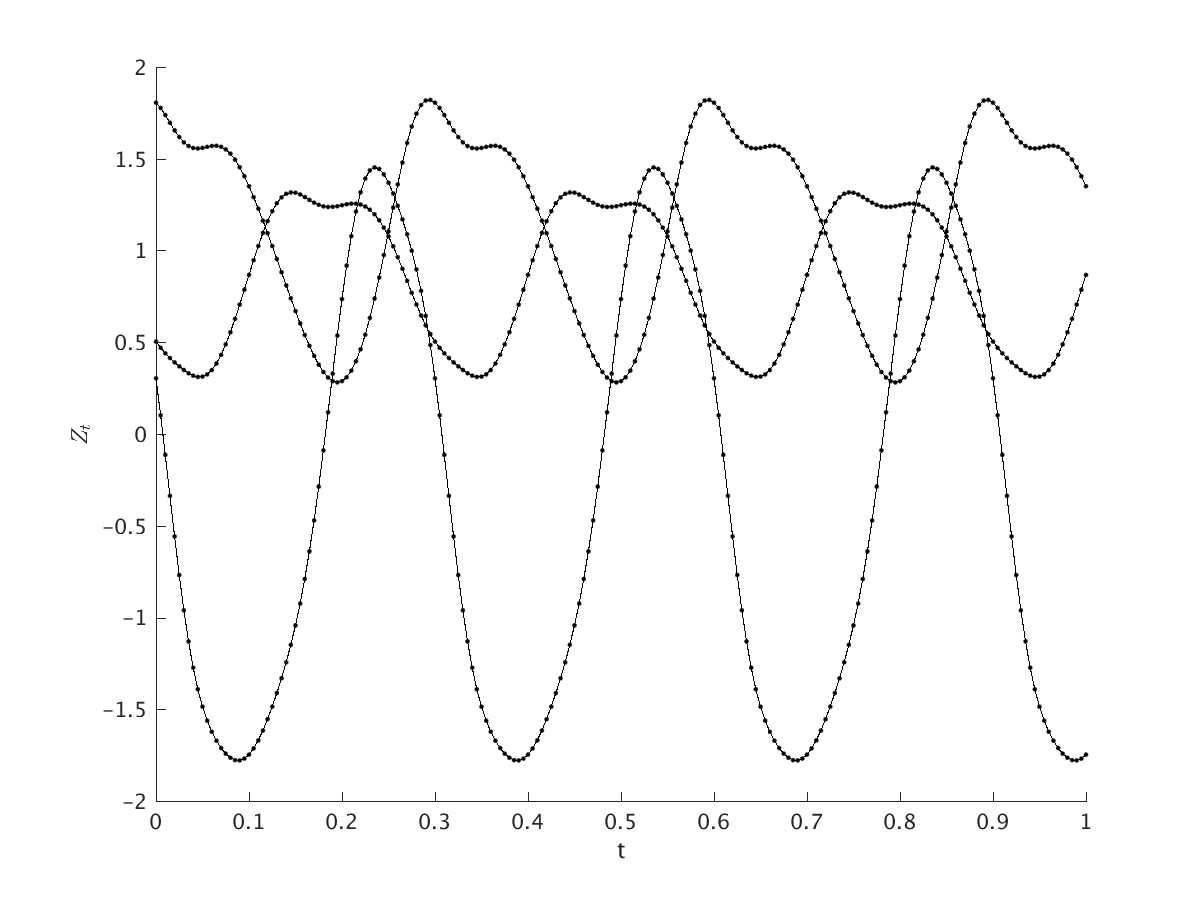
\includegraphics[scale=.5]{figures/per3.png}
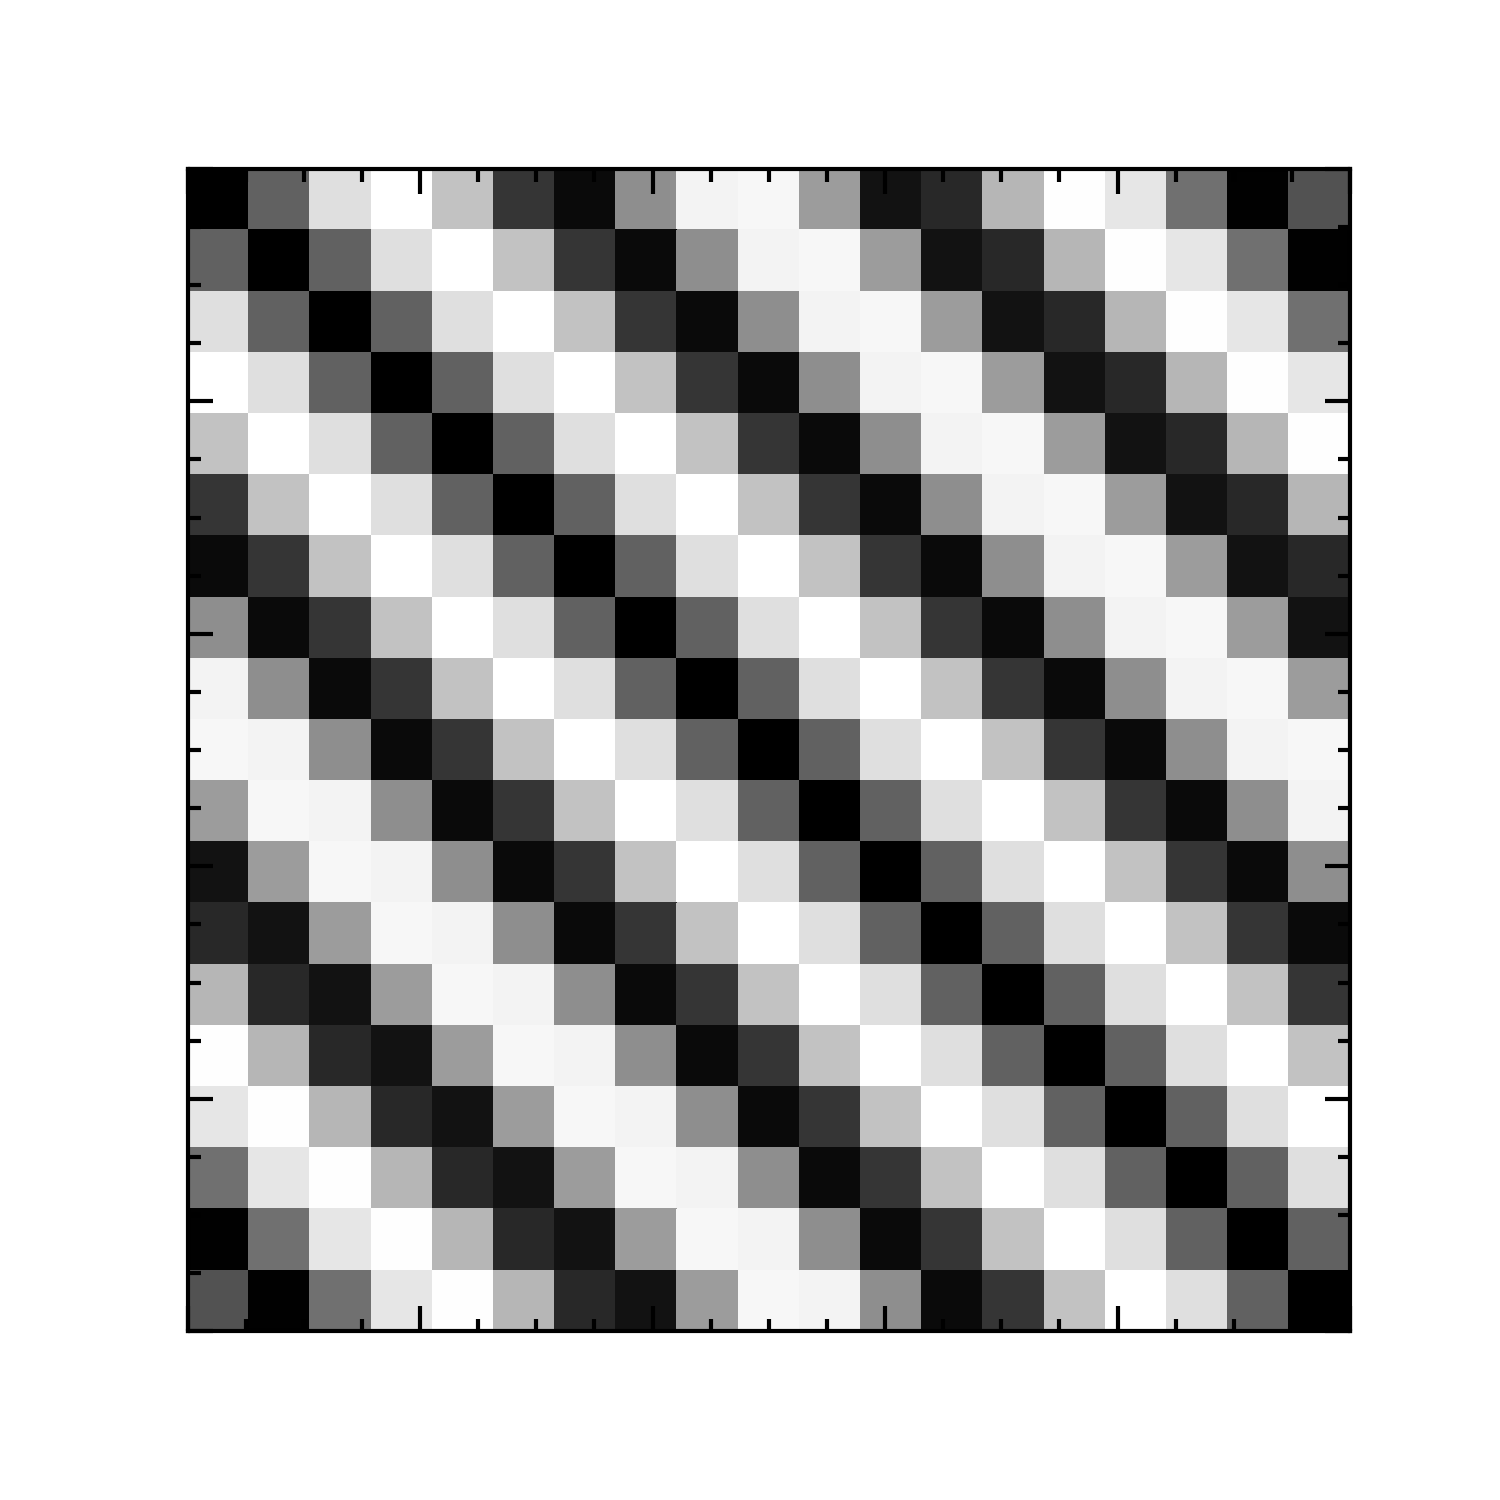
\includegraphics[scale=.4]{figures/covariancematrix_per.png}
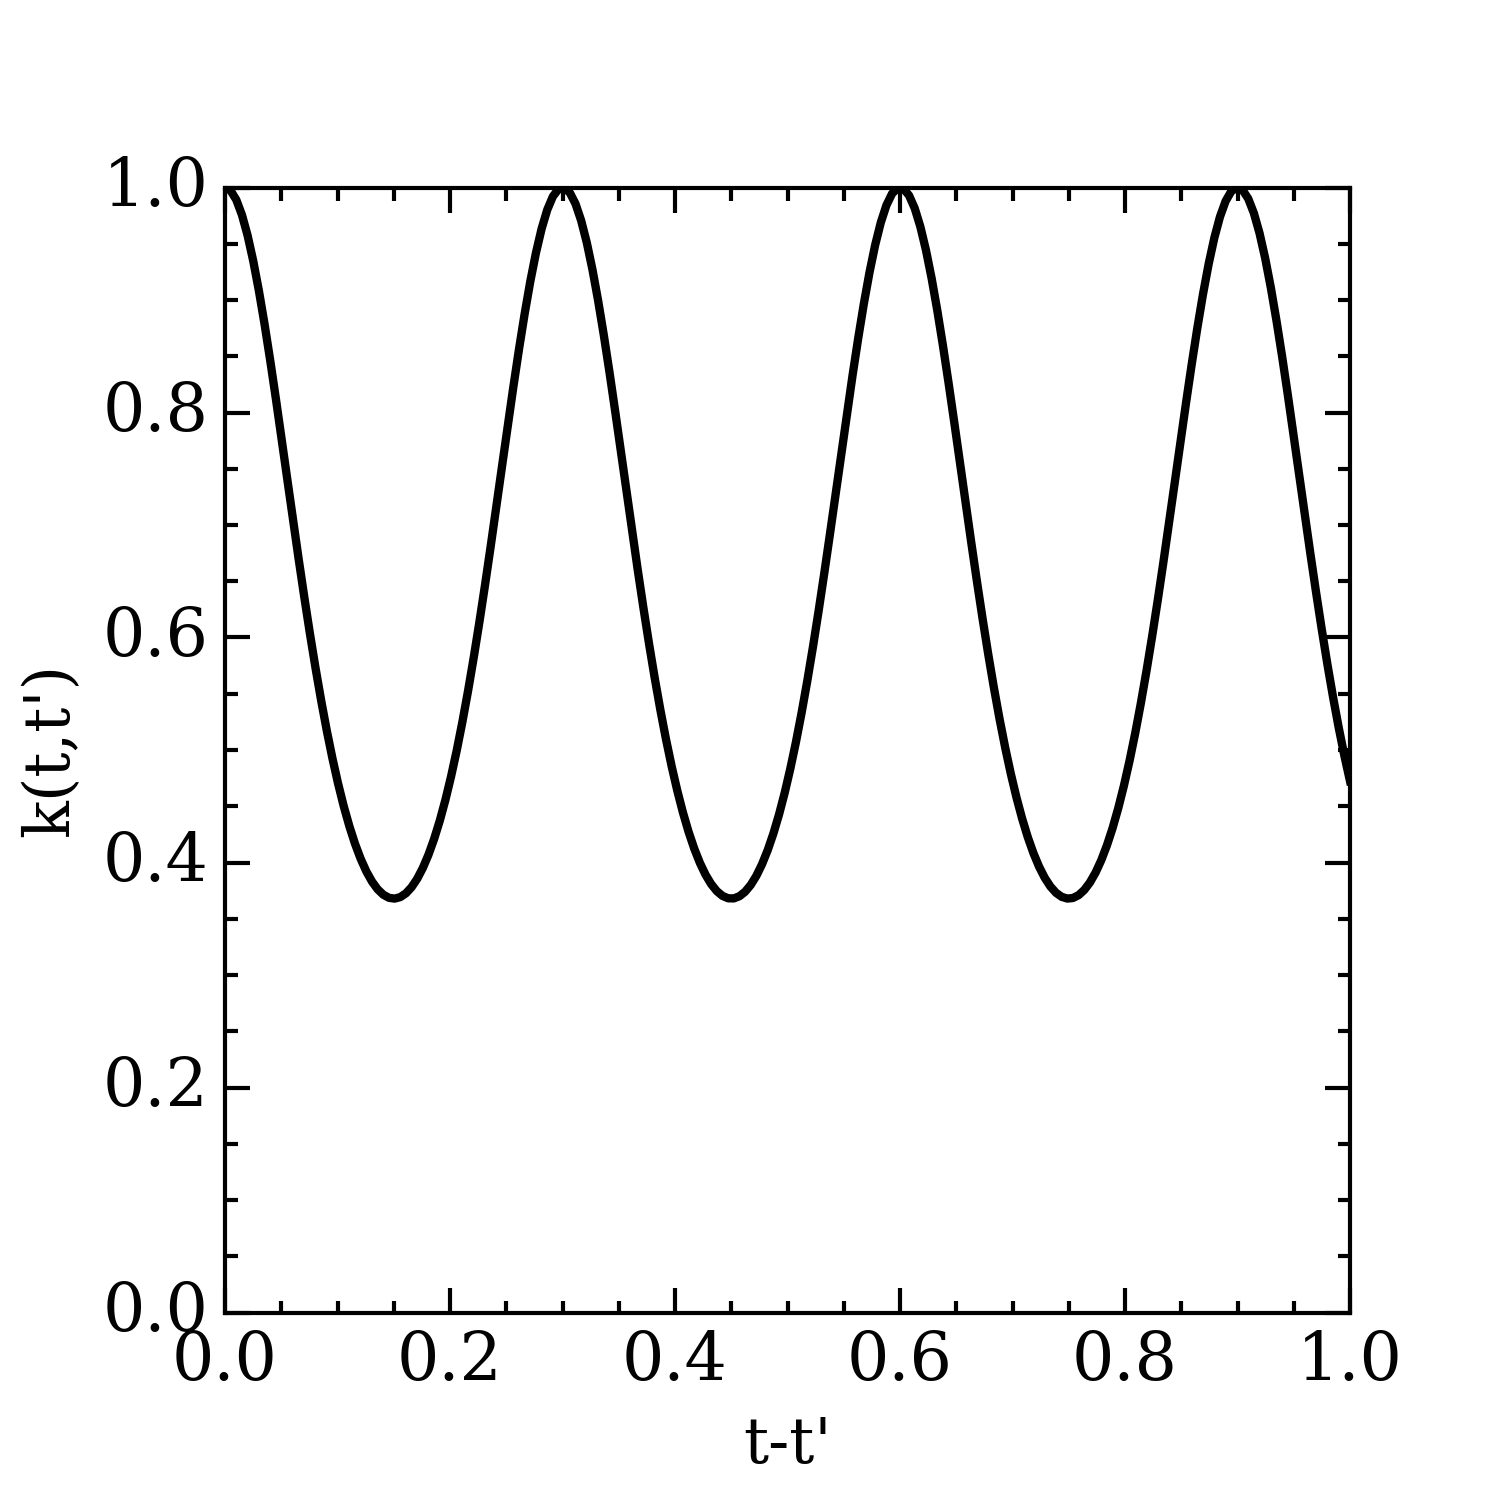
\includegraphics[scale=.4]{figures/kernel_per.png}
\caption{Same as Fig.~\ref{fig:sqexp} for a periodic covariance function. 
In all panels $\mathbf{\Theta} = \{a, \Gamma, P \}= \{1, 1, 0.3 \}$.
\label{fig:periodic}}
\end{figure}


\item \textbf{Quasi-Periodic}: this kernel combines the two preceding kernels to achieve 
a quasi-period behaviour with two competing timescales: $\lambda$ and $P$. This covariance 
function is often favoured when modelling stellar variability when the source of variability is 
rotationally modulated (hence the periodic term) but is not strictly periodic due to evolution of 
active regions' sizes and contrast. 
%\parencite[e.g.][]{vanderburg,  mancini, agnus, haywood14, grunblatt15}.
The covariance function is 

\begin{equation}
k(t_i,t_j) = a^2 \exp{\left( -\Gamma \sin^2{\left[ \frac{\pi |t_i-t_j|}{P} \right]} - 
\frac{|t_i-t_j|^2}{2\lambda^2} \right)}.
\label{eq:qpkernel}
\end{equation}

\noindent The coherence parameter $\Gamma$ can now be interpreted as the relative 
weighting of the periodic term to the squared exponential term. The quasi-periodic 
kernel 
therefore has four hyperparameters $\mathbf{\Theta} = \{a, \lambda, \Gamma, P \}$. Two 
samples from a GP with a quasi-periodic covariance function are shown in Fig.~\ref{fig:QP} 
along with the corresponding covariance matrix and kernel function.
\end{enumerate}

\begin{figure}
\centering
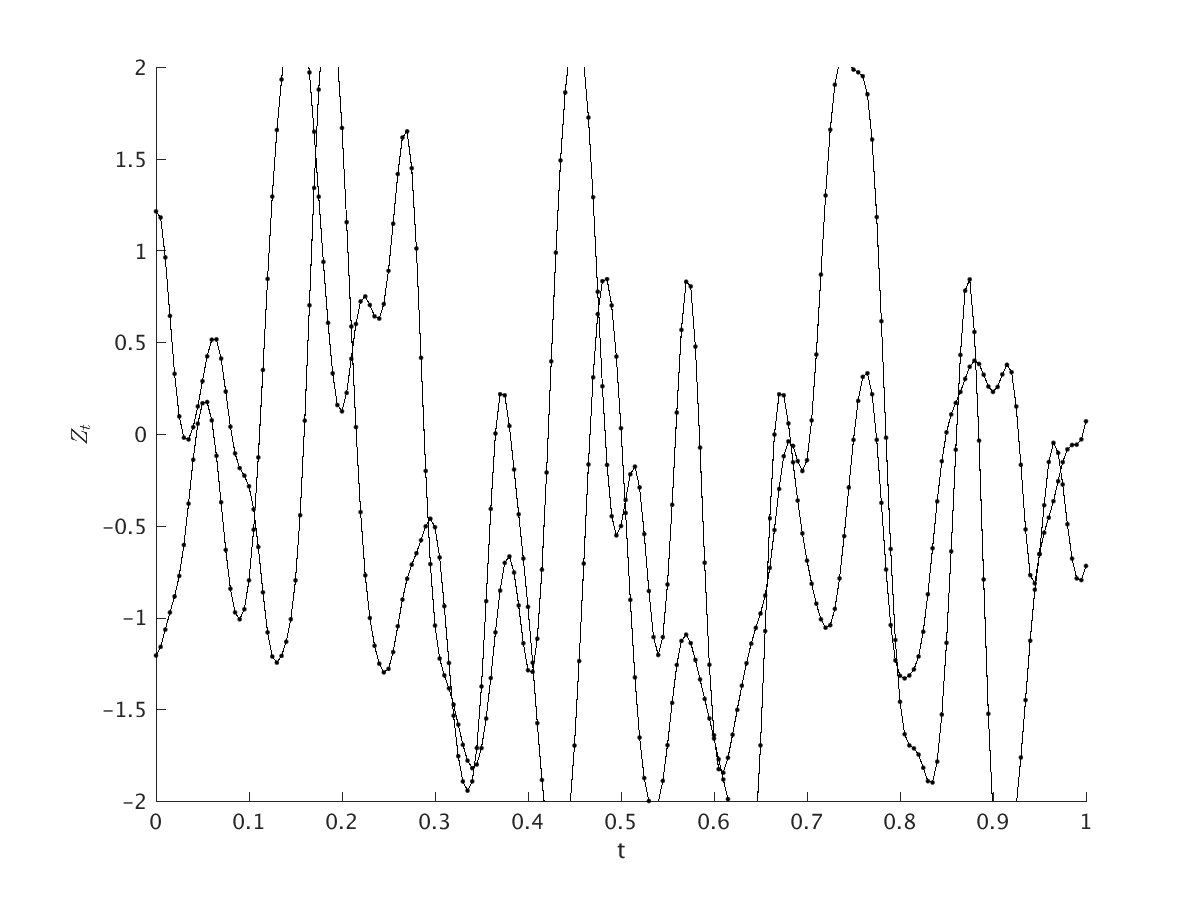
\includegraphics[scale=.5]{figures/qper2.png}
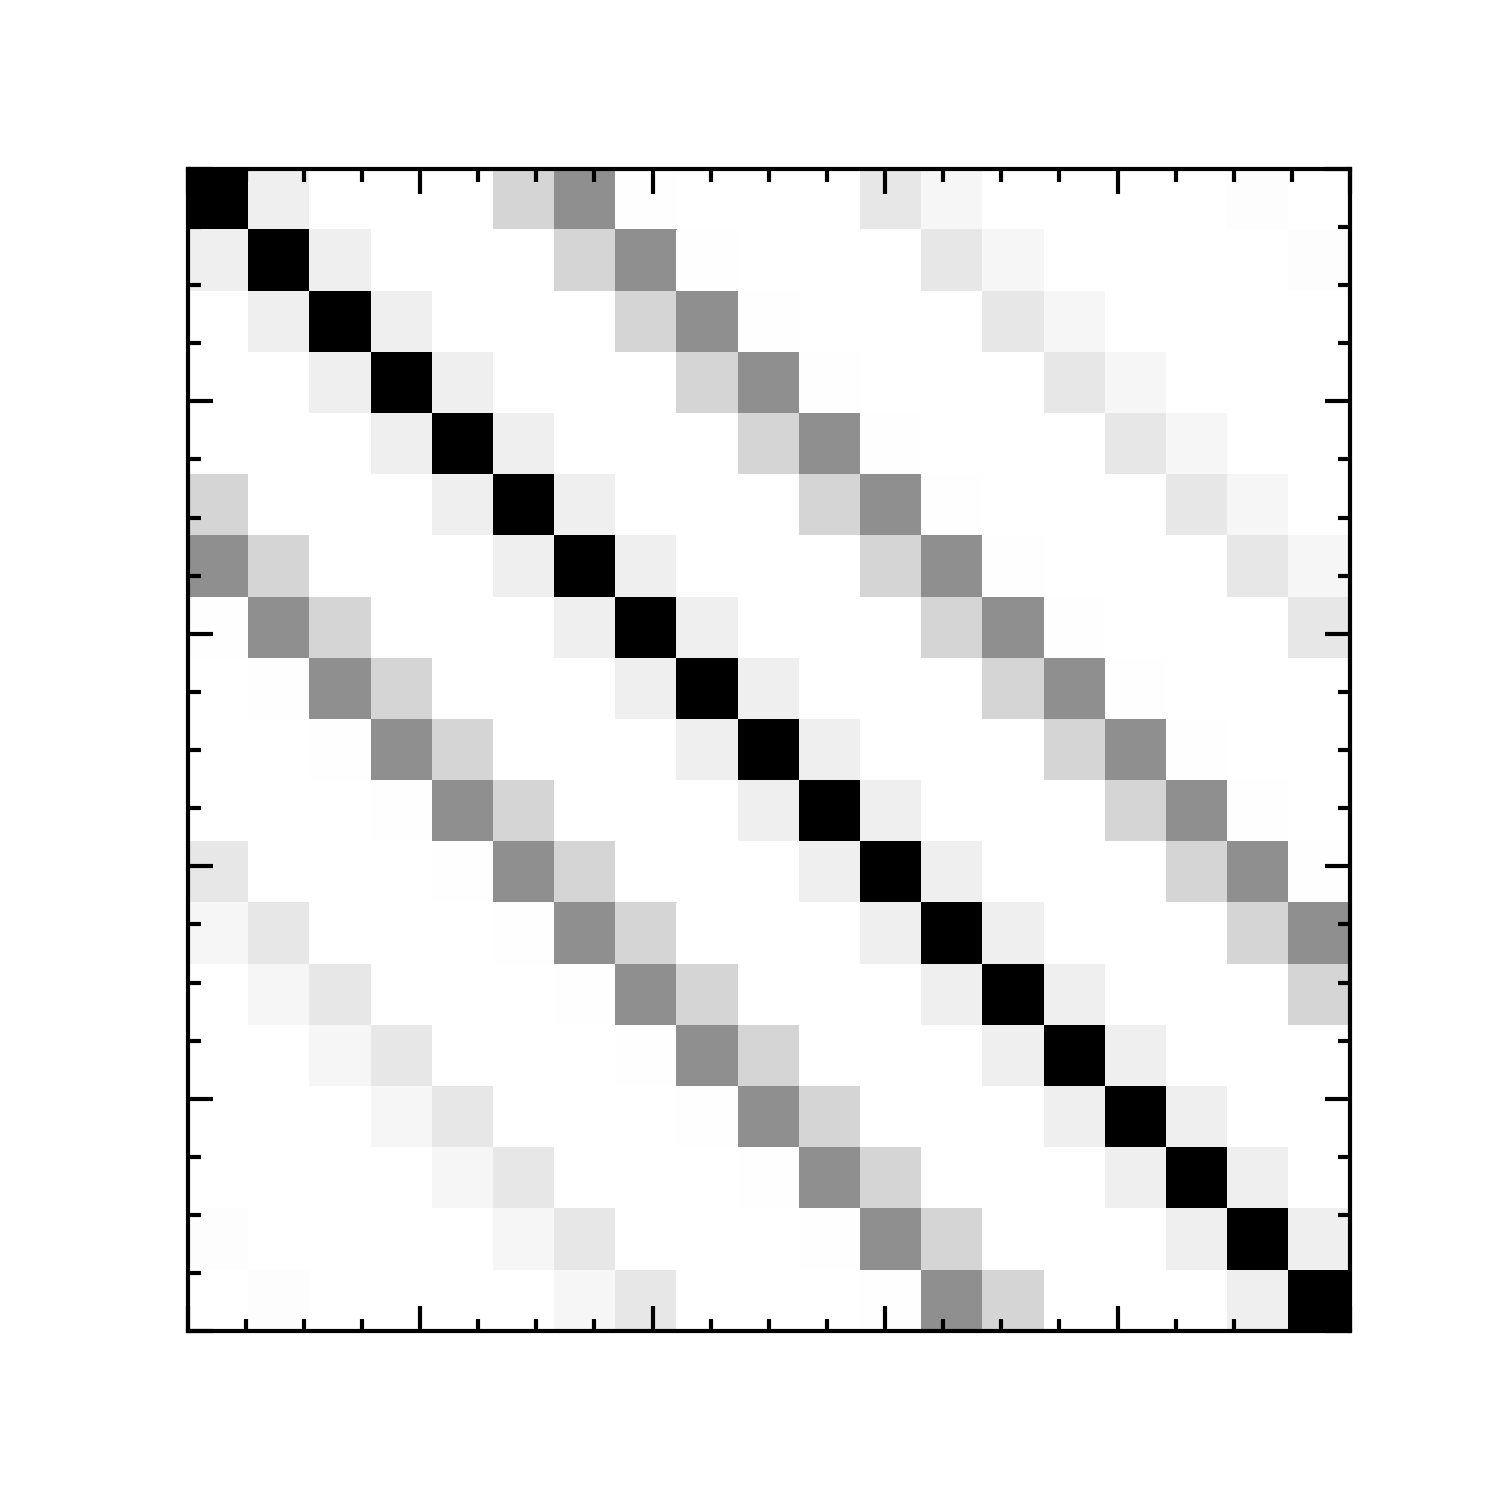
\includegraphics[scale=.4]{figures/covariancematrix_qper.png}
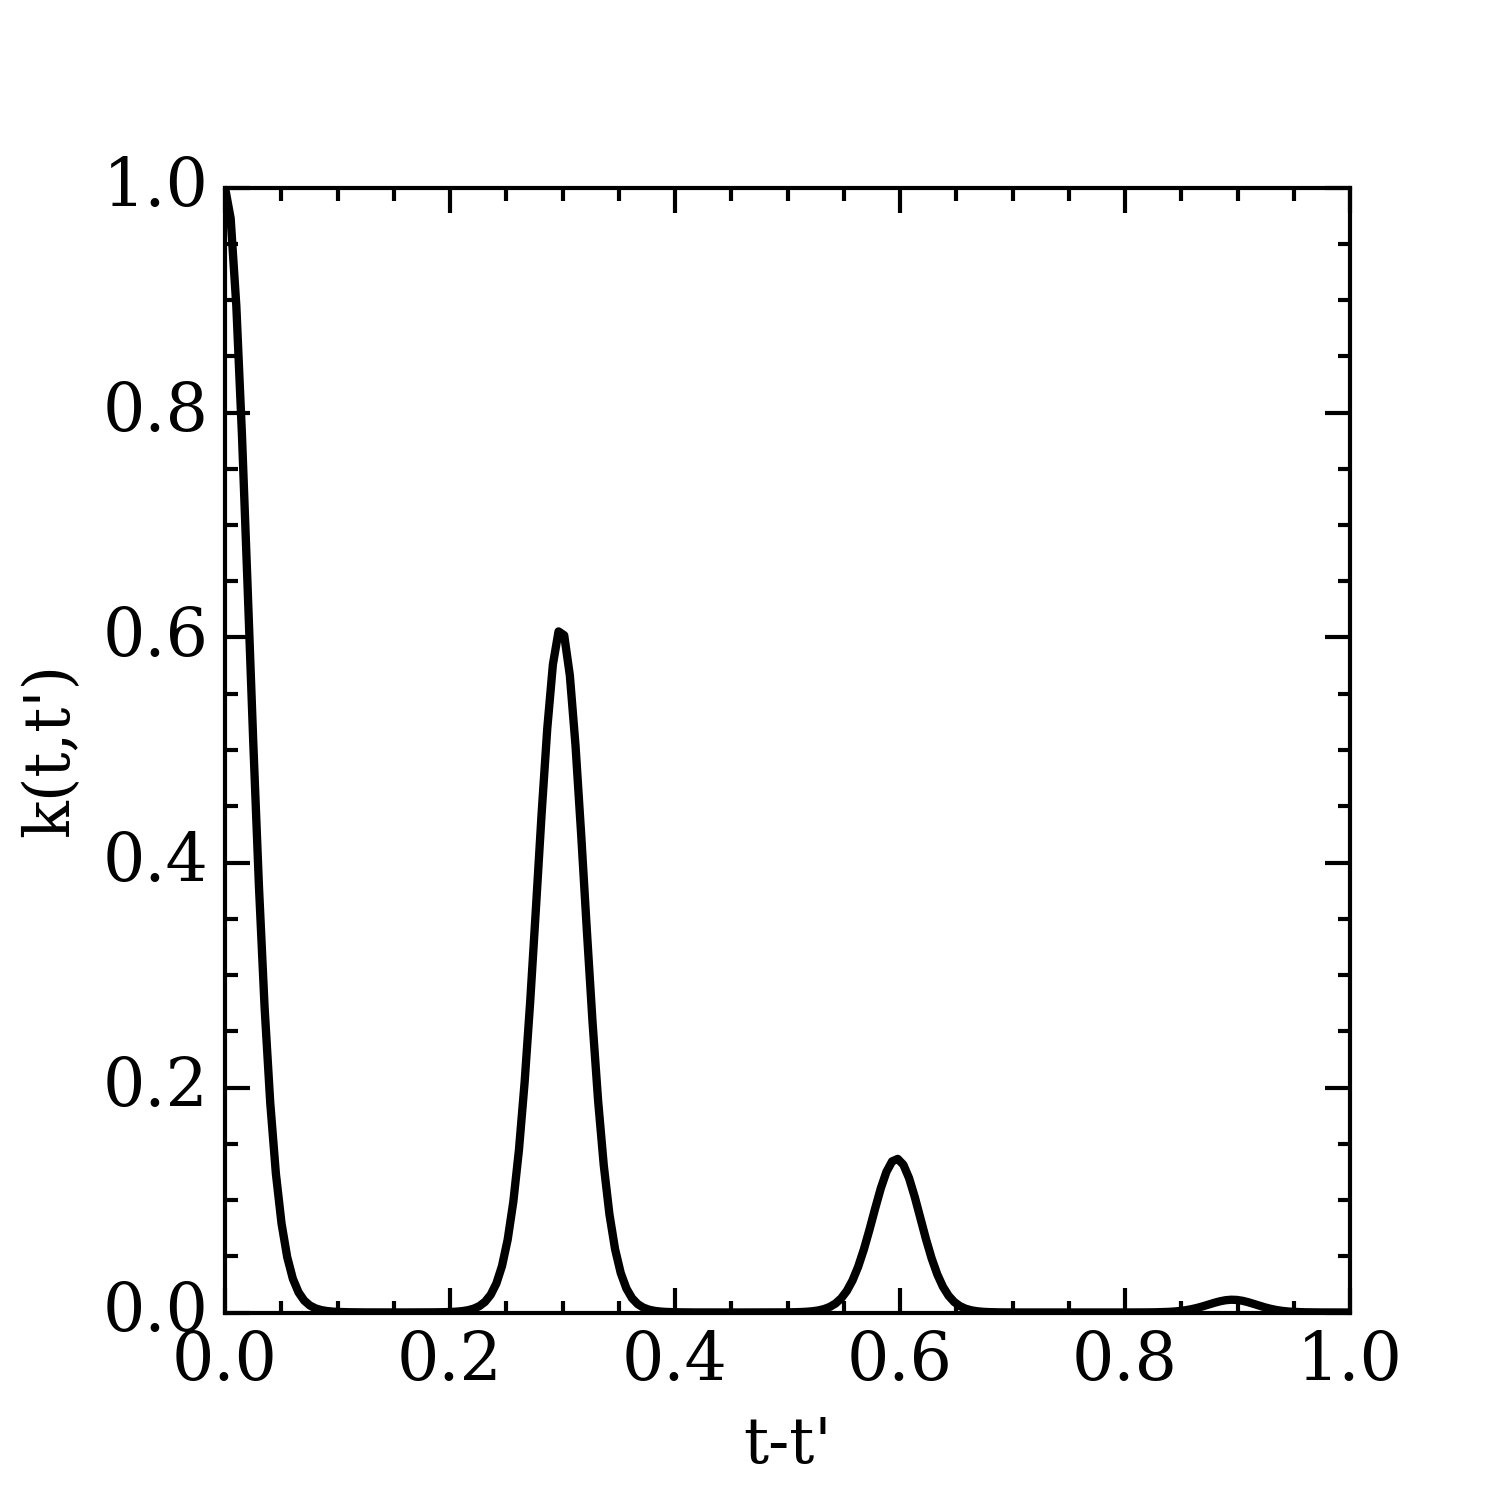
\includegraphics[scale=.4]{figures/kernel_qper.png}
\caption{Same as Fig.~\ref{fig:sqexp} for a quasi-periodic covariance function. 
In all panels $\mathbf{\Theta} = \{a, \lambda, \Gamma, P \}= \{1, 0.3, 10, 0.3 \}$.
\label{fig:QP}}
\end{figure}

\subsection{GPs \& RVs} \label{sect:gprv}
Let's elaborate more on the use of GPs as it pertains to modelling RV jitter. 
We wish to model the correlated (\emph{red}) noise arising from stellar jitter 
which the non-parametric GP formalism is well suited to. This is done 
through an appropriately chosen covariance kernel which is first 
\emph{trained} on 
an ancillary timeseries (not the RV measurements) which is sensitive to 
one or more sources of stellar jitter but is independent of the 
influence of planetary companions. A number of potential timeseries were 
discussed in Sect.~\ref{sect:diagnostics}. \\

%As has been done in small number of 
%studies so far \parencite[e.g.][]{haywood14, grunblatt15}, 
Training of the covariance kernel hyperparameters 
on the ancillary timeseries provides hyperparameter priors which are then 
applied to the evaluation of the RV timeseries plus a non-zero mean function equal 
to the number of planetary orbital solutions assumed in the system. 
\cite{grunblatt15} tested each of the latter three covariance kernels discussed 
above to model the photometric variability of the 
star Kepler-78 in its Kepler light curve. 
%They considered a squared exponential, 
%periodic, and quasi-periodic covariance functions (see Sect.~\ref{sect:covariance}). 
Using model selection methods based on the Bayesian information criterion (BIC) 
and Akaike information criterion (AIC), \cite{grunblatt15} found that the RV data 
favoured a keplarian component plus a quasi-periodic GP jitter model. Thus the 
predominant jitter signal in the data are likely rotationally modulated with a 
period equal to $P_{\mathrm{rot}}$. 
Indeed the GP is known to benefit substantially from \emph{a priori} knowledge of 
the stellar rotation period (Dumusque et al. \emph{in prep.}) 
which may be uncovered in the periodogram analysis of 
ancillary timeseries, particularly in high cadence photometry. Similar comparisons 
between different covariance functions applied to the photometric variability of 
stars have been 
conducted and also concluded that the best suited model is quasi-periodic 
\parencite[e.g.][]{angus15}. \\

Even being armed with an optimal covariance function there are still differing 
methods on how best to train the GP. What I have discussed so far has been 
demonstrated in a number of observational studies 
\parencite[e.g.][]{haywood14, grunblatt15}, namely the use of a single 
ancillary timeseries (often photometry) to train the GP. An alternative approach, 
outlined in \cite{rajpaul15}, involves training the GP simultaneously using multiple 
ancillary timeseries. This is a valid approach given that the former methodology 
treats a single ancillary timeseries as a GP and the linear combination of GPs and 
their derivatives is also a GP. Joint modelling of multiple ancillary timeseries 
assumes that each timeseries is a manifestation of a single underlying GP although 
constructing the corresponding $n(N \times N)$ covariance matrix $\mathbf{K}$, 
requires prescribing the covariance 
between each of the $n$ ancillary timeseries with one another. A task which is 
done in an admittedly inexact manner in \cite{rajpaul15} who test their formalism 
on the timeseries $\Delta$RV, $\log{R'_{\mathrm{HK}}}$, and BIS. \\

Recently, X. Dumusque hosted an RV challenge \parencite[part I in][]{dumusque16} 
in which he simulated a handful of planetary systems and 
computed the RV contribution from planetary companions, stellar jitter, and instrumental 
noise. He then constructed the corresponding 
RV, plus BIS, FWHM, and $\log{R'_{\mathrm{HK}}}$ timeseries. The data were then made 
available to the community who were asked 
to test their own algorithms on the timeseries and attempt to find and accurately 
detect as many planets as possible. 
Within the pool of participants in the RV challenge, two groups, each using one of the 
previously discussed GP approaches, submitted their results for evaluation. Among these 
two groups of GP enthusiasts was the so-called Oxford group from \cite{rajpaul15}. 
Through 
private discussions with X. Dumusque regarding the results of those teams, I was 
interested 
to hear that the group which did \emph{not} train on the timeseries 
simultaneously, actually outperformed the Oxford group despite not using all of the 
available data (see Fig.~\ref{fig:rvchallenge}). Given the difficulty in 
prescribing the covariance between each of these timeseries, the sensitivity of 
each timeseries to different physical sources of stellar jitter (see 
Sect.~\ref{sect:diagnostics}), and the apparent planet detection/characterization 
improvement 
when declining simultaneous GP training, I opt to train my GP model on a single 
ancillary timeseries at a time in my own GP code. \\

\begin{figure}
\centering
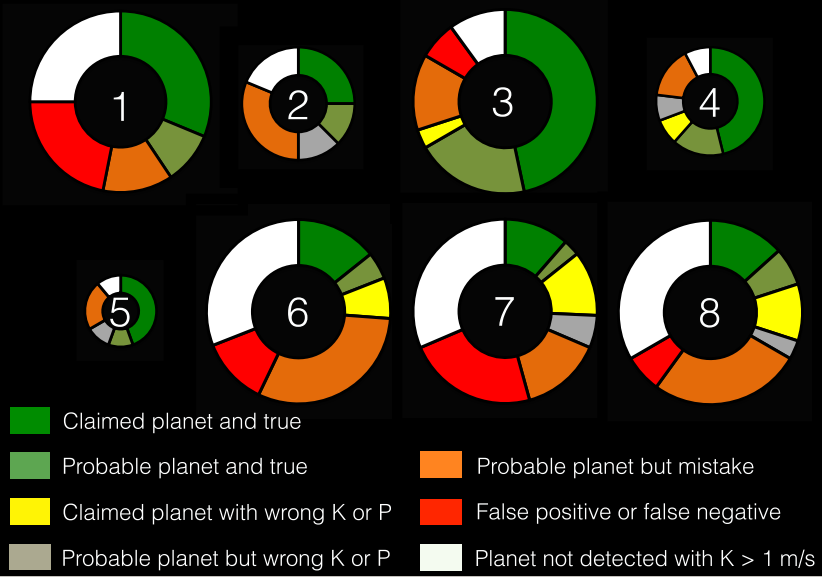
\includegraphics[scale=.4]{figures/rvchallenge.png}
\caption{A schematic depiction of the results of the RV challenge. The two groups 
of interest for the use of GPs are Groups 1 (Torino: GP training with a single 
timeseries) and 2 (Oxford: simultaneous GP training). The size of each 
group's circle is proportional to the number of systems analyzed. (Image credit: 
X. Dumusque) \label{fig:rvchallenge}}
\end{figure}

\subsection{Computing the GP model} \label{sect:bayes}
In general, when one has a model $\mathcal{M}$ 
that they are attempting to fit to a dataset of $N$ observations 
$\mathbf{y}$ taken at epochs $\mathbf{t}$, the quantity of interest is the marginalized 
posterior probability distributions of each model parameter. According to Bayes theorem, 
the posterior probability of the set of model parameters in the model $\mathcal{M}$ is 

\begin{equation}
\mathrm{P} (\mathbf{\Theta} | \mathbf{y}, \mathcal{M}) \propto \mathrm{P} (\mathbf{y} | \mathbf{\Theta}, \mathcal{M}) 
\cdot \mathrm{P} (\mathbf{\Theta}|\mathcal{M})
\end{equation}

\noindent where we are ignoring the normalization factor. In order to obtain each model 
parameter's posterior probability distribution, marginalized 
over all other model parameters, we must first compute the model parameter prior 
$\mathrm{P}(\mathbf{\Theta}|\mathcal{M})$ (see Sect.~\ref{sect:priors})
and the value of the likelihood function 
$\mathcal{L} \equiv \mathrm{P} (\mathbf{y} | \mathbf{\Theta},\mathcal{M})$ given a unique set of 
model parameters $\mathbf{\Theta}$. \emph{The likelihood $\mathcal{L}$ is an objective function 
to be maximized and represents 
the probability of obtaining the observed values $\mathbf{y}$ given a model $\mathcal{M}$ 
and unique set of model parameters $\mathbf{\Theta}$.} 
The most generalized expression of the logarithmic likelihood function\footnote{We commonly 
work in natural logarithmic units.} is 

\begin{equation}
\ln{\mathrm{P}(\mathbf{y} | \mathbf{\Theta},\mathcal{M})} = -\frac{1}{2} \left( \mathbf{r}^{\mathrm{T}} 
\mathbf{K}^{-1} \mathbf{r} + \log{\mathrm{det} \mathbf{K}} + N \log{2\pi} \right).
\label{eq:lnlike}
\end{equation}

\noindent Recall that $\mathbf{r}=\mathbf{y}-\boldsymbol{\mu}$ 
is the residual $N$-vector and $\mathbf{K}$ is the $N \times N$ covariance matrix 
computed with Eq.~\ref{eq:Kmatrix}. 
In Eq.~\ref{eq:lnlike}, the first term represents the extent to which the observed data 
$\mathbf{y}$ match the model $\boldsymbol{\mu}$; the goodness-of-fit measurement. The second 
term implements ``Occam's razor'' by penalizing overly complex models of the covariance and 
the final term is the normalization constant. \\

In order to compute the marginalized posterior probability distributions, we use a Markov 
chain Monte Carlo method. The description of the details of this analysis are deferred to 
Sect.~\ref{sect:mcmc}. 

\subsubsection{Priors} \label{sect:priors}
Computing $\mathrm{P} (\mathbf{\Theta} | \mathbf{y}, \mathcal{M})$ also requires the prior 
probability of the set of model parameters $\mathrm{P} (\mathbf{\Theta} | \mathcal{M})$. 
Assuming that all model parameters are independent, the total prior can be expressed as 
the product of the priors computed for each model parameter %$\theta_i \in \mathbf{\Theta}$ 
based on any prior knowledge we have regarding the value of that parameter 
\parencite{gregory05}. \\

Unfortunately, it is often the case that we have very little 
prior information regarding the value of most model parameters. In such cases, the form 
of the adopted prior must be \emph{uninformative} such that the prior does not favour 
any small range of particular parameter values but may still be used to 
impose objective conditions 
such as the sign of the parameter or its upper and lower limits. One commonly used 
uninformative prior on an arbitrary model parameter $\theta$ is the 
\emph{Jeffreys prior} \parencite{gregory07} 

\begin{equation}
\mathrm{P} (\theta | \mathcal{M}) = \frac{1}{\theta \ln{(\theta_{\mathrm{max}} / 
\theta_{\mathrm{min}})}},
\end{equation}

\noindent parameterized by the upper and lower limits of the parameter 
($\theta_{\mathrm{max}}$ and $\theta_{\mathrm{min}}$ respectively). 
The Jeffreys prior is a popular uninformative prior for unknown parameters 
which follow a logarithmic scale such as timescales which are 
not constrained by significant 
peaks in the frequency spectrum of a set of observations (e.g. $P$). The Jeffreys prior 
applied to timescales such as $P$ allows us to sample $P$ more sparsely at long 
periods than at short ones and therefore obtain an unbiased sample over the 
full range of $P$ which spans multiple orders of magnitude (i.e. scale 
invariance). \\

Another popular uninformative prior is the \emph{modified Jeffreys prior} 
\parencite{gregory07}

\begin{equation}
\mathrm{P} (\theta | \mathcal{M}) = \frac{1}{\theta+\theta_0} 
\frac{1}{\ln{(1+\theta_{\mathrm{max}}/\theta_0)}},
\label{eq:modjeff}
\end{equation}

\noindent wherein for $\theta \ll \theta_0$ ($\theta_0$ is the `knee' of the 
distribution), Eq.~\ref{eq:modjeff} behaves like 
a \emph{non-informative} uniform prior and for $\theta \gg \theta_0$ it behaves 
like a Jeffreys prior. $\theta_{\mathrm{max}}$ is again the upper bound on the values 
of $\theta$. \\

However, there are cases in which some prior knowledge regarding a model parameter 
value is know. For example, let's say that a new transiting exoplanet 
is discovered and we wish to perform follow-up observations of its host star's radial 
velocity. The detection of multiple transit events provides prior knowledge on the 
planet's orbital period $P$ and time of mid-transit T0 (orbital phase), often to 
high accuracy. Modelling of 
the planet's ephemeris from the transit light curve will provide \emph{most likely} 
values of $P$ and T0 along with their respective uncertainties. 
When fitting the RV model 
we can use this introduce this extra information into the calculation 
by replacing the uninformative priors on $P$ and T0 with 
more restrictive priors such as a Gaussian prior with mean and standard deviation given 
by the reported measurements of $P$ and T0 and their uncertainties. 

%When using the GP formalism to model the covariance between measurements, the 
%covariance matrix $\mathbf{K}$ is described by 

\section{Markov chain Monte Carlo} \label{sect:mcmc}
As we saw in Sect.~\ref{sect:bayes}, we are interested in computing the 
marginalized posterior probability distributions of the parameters of our model. 
In Sect.~\ref{sect:gprv} we saw that one set of model parameters contains 
the hyperparameters of our adopted GP model 
of the stellar jitter which is first \emph{trained} on an ancillary timeseries before 
being applied to a GP fit of the observed radial velocities with a non-zero 
mean function (instead we use Eq.~\ref{eq:keps} to compute the mean function). 
To obtain the most likely 
model parameters and their uncertainties we use a Markov chain Monte Carlo 
(MCMC) routine 
to sample each parameter's posterior probability distribution based on the model 
likelihood (Eq.~\ref{eq:lnlike}) and parameter prior probabilities (see 
Sect.~\ref{sect:priors}). 
The matrix inversion and determinant calculations required to compute the logarithmic 
likelihood in the MCMC is done using a Cholesky decomposition. This method exploits the 
nature of the covariance matrix $\mathbf{K}$ being symmetric and positive semidefinite 
and is more efficient than other numerical methods of solving the system 
of linear equations $\mathbf{K} \mathbf{x} = \mathbf{b}$. 

\subsection{Model construction}
As discussed, to obtain the desired result of a planetary RV model which is contaminated 
by stellar jitter, two MCMCs are used. The first MCMC is performed on the 
ancillary timeseries used for \emph{training}. Here the MCMC samples the marginalized 
posterior probabilities of the GP hyperparameters. 
Recall that a quasi-periodic covariance function was chosen earlier. 
%Following a number of observational 
%studies using GPs to characterize planetary signals 
%\parencite[][]{haywood14, grunblatt15, mancini15, vanderburg15}, 
%we adopt a quasi-periodic (Eq.~\ref{eq:qpkernel}) 
%covariance kernel. 
At first glance this assumption appears to be a reasonable choice given that 
the strong components to the stellar jitter in M-dwarfs arises from active regions 
which are rotationally modulated but evolve over time and are therefore not strictly 
periodic. In this case we use an MCMC to measure the four GP hyperparameters 
(Eq.~\ref{eq:qpkernel}) with the inclusion of an extra error term $s$ to be added in quadrature  
to each measure uncertainty ($\sigma_i \to \sqrt{\sigma_i^2 + s^2}$) 
to adjust the overall measurement uncertainty for cases 
in which the input measurement uncertainties are underestimated. 
Therefore the factor of $s$ only contributes to the diagonal elements of $\mathbf{K}$.  
The set of five GP hyperparameters is then 
$\mathbf{\Theta}_{\mathrm{GP}}=\{a,\lambda,\Gamma,P_{\mathrm{rot}},s\}$. \\

The marginalized posterior distributions on the hyperparameters in 
$\mathbf{\Theta}_{\mathrm{GP}}$ are then used as 
custom prior probability distributions when modelling the RV measurements 
with a GP plus $N$ keplarian solution. According to the equation for the keplarian 
RV solution (Eq.~\ref{eq:rv}), there are six parameters to fit; 
$\mathbf{\Theta}_{\mathrm{RV}} = \{P,\mathrm{T}0,V_0,K,e,\omega\}$. As a reminder these are 
the star/planet's orbital period, reference epoch, stellar systemic velocity, 
RV semiamplitude, orbital eccentricity, and argument of periastron. 
This second MCMC, this time on the RV measurements, therefore has eleven model 
parameters; $\mathbf{\Theta}_{\mathrm{GP}} \cup \mathbf{\Theta}_{\mathrm{RV}}$. \\

We note that in order to reduce the bias towards high-eccentricity orbits when fitting 
the parameters $\{e, \omega \}$ directly, especially in low-eccentricity orbits, following 
\cite{ford06} we define two new parameters 

\begin{align}
h &= \sqrt{e} \cos{\omega}, \\
k &= \sqrt{e} \sin{\omega}.
\end{align}

\noindent Fitting $h$ and $k$ reduces the joint posterior correlation between 
$e$ and $\omega$ and 
by taking the square root of $e$, helps mitigate the bias of RV fits towards 
high-eccentricity orbits. Together, the \emph{maximum a posteriori} (MAP) values of $h$ 
and $k$ can be used to compute the MAP values of $e=h^2 + k^2$ and $\omega=\arctan{(k/h)}$. 

\subsection{Prior selection}
The choice of GP hyperparameter priors are summarized in Table~\ref{table:priors}. 
The choices are mostly based on the adopted priors from the 
HARPS RV team with the exception of the timescale of the 
periodic term $P$ whose prior is uniform, like the HARPS adaptation, but whose 
limits we restrict to the apparent stellar rotation period found via a Lomb-Scargle 
periodogram analysis of the ancillary timeseries. The width of the uniform distribution 
is conservatively chosen 
to extend well beyond the width of the periodogram peak because such peaks are known 
to be inexact. \\

\begin{threeparttable}
\caption{Adopted Quasi-Periodic GP plus Keplarian Model Parameter Priors}
\label{table:priors}
\begin{tabular}{cc}
  \hline
  \hline
  \textbf{Parameter} & \textbf{Prior} \\
  \hline
  & \\
  \multicolumn{2}{c}{\textbf{GP Hyperparameters}} \\
  \hline
  $a$ & Uniform \\
  $\lambda$ & Jeffreys \\
  $\Gamma$ & Jeffreys \\
  $P$ & Uniform \\
  $s$ & Jeffreys \\
  \hline
  & \\
  \multicolumn{2}{c}{\textbf{Keplarian Model Parameters}} \\
  \hline
  $P$ & Jeffreys/Gaussian\tnote{a} \\
  T0 & Uniform \\
  $V_0$ & Uniform \\
  $K$ & Modified Jeffreys \\
  $C_k$ & Uniform \\
  $S_k$ & Uniform \\
  \hline
  \end{tabular}
\begin{tablenotes}
\item[a] Jeffreys when searching for orbital periods `blindly' and 
Gaussian when the orbital period is known from, say, the planets 
transit light curve.
\end{tablenotes}
\end{threeparttable}


\subsection{Running the MCMC}
To sample the posterior probability distributions of the model parameters, we use a python 
implementation of the affine-invariant MCMC ensemble sampler from \cite{goodman10}. The code 
is called \texttt{emcee} and is detailed in \cite{foremanmackey13}. The affine-invariant 
ensemble sampler is a favourable algorithm over the commonly used Metropolis-Hastings sampling 
algorithm because of its efficiency. Ensemble sampling can generally produce independent samples 
of the target probability density with a much shorter autocorrelation 
time\footnote{\textbf{autocorrelation time}: the number of steps in the Markov chain to 
draw independent samples of a parameters target probability density.} than 
Metropolis-Hastings. \\
 
The ensemble sampler works by initializing two sets of walkers $S^0$ and $S^1$. Walkers can be 
thought of as parallelized Markov chains whose positions are correlated with the positions 
of other walkers. Each set $S^i$ 
contains $K/2$ walkers at specified initial `positions' $X_k$ in the $n$-dimensional parameter 
space where $n$ is the number of parameters in $\mathbf{\Theta}$ 
and $k$ is the walker index from $1,\dots,K$. 
The two sets can be written as $S^0 = \{X_k, \forall k=1,\dots,K/2\}$ and 
$S^1 = \{X_k, \forall k=K/2+1,\dots,K\}$. In my work, the position of each walker is 
initialized in a Gaussian ball around an initial `guess' of the $\mathbf{\Theta}$ parameter 
values. The $n$ means and widths of the Gaussian ball are left as hyperparameters of the MCMC 
and are discussed in Sect.~\ref{sect:mcmcparams}. 
Following the initialization of all $K$ walkers, we attempt to update the position 
of the $k^{\mathrm{th}}$ walker in $S^0$, $X_k$, by randomly drawing a walker at position 
$X_j$ from the 
other set $S^1$ and proposing a new position $X_k^{'} \to X_j + Z(X_k-X_j)$ where $Z$ is a 
random variable drawn from the distribution $g(z)$ whose form is proposed to be 

\begin{equation}
g(z) \propto 
\begin{cases}
\frac{1}{\sqrt{z}} & \quad \text{if } z \in \left[ \frac{1}{a}, a \right], \\
0 & \quad \text{otherwise}  \\
\end{cases} 
\label{eq:gprob}
\end{equation}

\noindent in \cite{goodman10}. The scale parameter is set to the default value 
$a=2$ in the \texttt{emcee} code. We shall see in Sect.~\ref{sect:mcmcparams} 
how the MCMC hyperparameter 
$a$ can be modified to ensure adequate sampling of the target posterior probability 
distributions. \\

Not all steps proposed by the aforementioned algorithm 
are accepted. When attempting to update the walker position from 
$X_k \to X_k^{'}$, the proposed step is only accepted if the probability $q \geq r$ 
where

\begin{equation}
q = \min{\left( 1, Z^{n-1} \frac{\mathrm{P}(X_k^{'})}{\mathrm{P}(X_k)} \right)}
\end{equation}

\noindent and $r$ is a random variable drawn from a uniform distribution on the 
unit interval; $r \sim \mathrm{U}(0,1)$. If the proposed step for $X_k$ is accepted then $X_k$ is 
set to the proposed position $X_k^{'}$, else, $X_k$ is left unchanged until the next 
step in the chain. These proposed steps are computed simultaneously for all $K/2$ walkers 
in $S^0$ using the walkers in $S^1$. 
The same is then done for the $K/2$ walkers in $S^1$ using the recently updated walkers in 
$S^0$. The full procedure 
is then repeated for as many steps in the chain as is specified by the user at 
initialization. This walker updating 
scheme is referred to as the \emph{parallel stretch move} 
and allows the each walker's `Markov 
chain' to be completed rapidly compared to other MCMC sampling methods. \\

\subsection{Ensuring convergence}
To ensure that the MCMC has done an adequate job of sampling the target probability 
densities, we must test the convergence of the algorithm. 
The first test of convergence is done at the end of the chain by calculating $a_f$: the 
fraction of proposed steps which are accepted. A very low acceptance fraction 
may mean that the target posterior probability is multi-modal with modes separated by 
broad `valleys' such that the ensemble sampler gets stuck in one of the high probability 
modes. In general, a small $a_f$ means 
that the chain has done a very poor job at exploring the target probability 
density and MAP parameter values will be mistaken while each parameter's uncertainty 
estimation will be underestimated. Conversely, 
too high an acceptance fraction implies that the chain is behaving as a random walk thus 
not sampling the full extent of the 
target probability density. Although there is no generally agreed upon 
value of $a_f$, I take $a_f \in [0.2,0.6]$ to be the range of acceptable values. \\

The second convergence 
test is the autocorrelation time which directly measures the number of steps 
required to obtain independent samples of the target probability density. We saw previously 
that the affine invariant ensemble sampler is a favourable MCMC sampling algorithm because 
of its short autocorrelation time. For our purposes of estimating model parameter 
uncertainties, it is suggested that we only require a few independent samples obtained 
over say 10 autocorrelation times. The length of each walker's chain may be extended 
if their previously set length is found to be $\lesssim 10$ autocorrelation times.

\subsection{MCMC hyperparameters} \label{sect:mcmcparams}
We have seen so far a number of MCMC hyperparameters which must be specified by the user 
in order to run an MCMC ensemble sampler on an input dataset. These hyperparameters will control 
whether or not an MCMC converges and are typically determined by monitoring the MCMC 
performance on a given dataset and analyzing the resulting parameter posterior samples. 
Modifications to the hyperparameters can then be made if the MCMC does not perform adequately 
after its first attempt. \\

In no particular order, the hyperparameters to be adjusted by the user are 

\begin{enumerate}
\item \textbf{The number of walkers $K$.} It has been 
suggested by \cite{foremanmackey13} that there is no mathematical reason why this number should 
not be as large as possible aside the performance issues that will undoubtedly arise for very 
large values of $K$. I typically 
assign $K=100$. Increasing $K$ can improve the acceptance fraction if it is found to be 
too low. 
\item \textbf{The scale parameter $a$,} 
seen in Eq.~\ref{eq:gprob}, can be used to modify the acceptance fraction 
via increasing or decreasing the threshold probability $q$ of accepting steps in the chain. 
Decreasing the scale parameter to values less than the default value ($a<2$) results in an increase 
in $q$ and consequently an increase in the acceptance fraction. Similarly, increasing $a$ can lower 
the acceptance fraction.
\item \textbf{The initialization of the walkers} is done by specifying initial positions of each 
walker in a Gaussian ball in the $n$-dimensional parameter space. The Gaussian ball has a $n$-vector 
mean, equal to the initial guess of each parameter's value, and $n$-vector standard deviation 
whose entries are chosen to be comparable to how well a parameter's value is thought to be known 
given the dataset. 
For instance, if when looking at a RV timeseries which has an apparent semiamplitude of 
$K = 10 \pm 5$ \mps{} (not to be confused with the number of walkers $K$) potentially attributed to a 
planetary companion, my initialization of the walker in the $K$ dimension will be a Gaussian with 
$(\mu, \sigma)=(10,5)$ \mps{.} The size of the Gaussian ball will affect how long it takes the walkers 
to explore the parameter space and settle into any regions of high likelihood.
\item \textbf{The chain length} or number of steps in the chain can be used to ensure that a sufficient 
number of independent samples of the target probability density are evaluated. The chain length is 
determined 
after a preliminary MCMC is run from which the autocorrelation time is calculated. The final chain 
length is then chosen to be at least ten autocorrelation times.
\item \textbf{The \emph{burn-in} length} represents the first steps in a Markov which allow the 
parameter space to be reasonably explored before a second Markov chain is run for the purpose of 
parameter uncertainty estimation. The burn-in 
length should also be a few autocorrelation times and is 
therefore determined after a preliminary MCMC, similar to the chain length's determination. 
\end{enumerate}


\section{Point-form Thesis: Radial Velocity Modelling with Gaussian Processes}
\begin{itemize}
\renewcommand\labelitemi{--}
\item~\ref{sect:gpintro} \textbf{Introduction to Gaussian Processes (GPs)}: GP regression  
is a non-parametric supervised learning technique which is well-suited to modelling the 
effects of stellar jitter in radial velocity timeseries using ancillary observable timeseries.
\item~\ref{sect:gpformalism} \textbf{GP Formalism}: the method works by chosing a covariance 
function to model how data are correlated with one another and optimzing the hyperparameters 
of that function via likelihood maximization. 
\item~\ref{sect:mcmc} \textbf{Markov chain Monte Carlo}: use the affine invariant ensemble 
sampling method in Markov chain Monte Carlo simulations to model the \emph{trained} GP model 
and the GP plus keplarian model of the observed radial velocities.  
\end{itemize}
